%%%%%%%%%%%%%%%%%%%%%%%%%%%%%%%%%%%%%%%%%%%%%%%%%%%%%%%%
% Template:      Talleres Latex
% Document:      Formato de talleres
% Version:       DEV
% Codificacion:  UTF-8
% Autores:       Angel David Barraza Mercado
% Correos:       angel.barrazamer@campusucc.edu.co
% Institucion:   Universidad Cooperativa de Colombia - Campus Monteria
% Departamento:  Ingenieria de Sistemas
% Fecha:         Segundo periodo academico del 2026
%%%%%%%%%%%%%%%%%%%%%%%%%%%%%%%%%%%%%%%%%%%%%%%%%%%%%%%%

\documentclass[12pt,a4paper]{report}

% Paquetes a importar
\usepackage[utf8]{inputenc}
\usepackage[T1]{fontenc}
\usepackage[spanish]{babel}
\usepackage{lmodern}
\usepackage{parskip}
\usepackage{amsmath,mathrsfs}
\usepackage{amsfonts}
\usepackage{amssymb}
\usepackage{makeidx}
\usepackage{graphicx}
\usepackage{float}
\usepackage{geometry}
\usepackage{multicol}
\usepackage{bbding}
\usepackage{xcolor}
\usepackage{lipsum}
\usepackage{xparse}
\usepackage{titlesec}


% Definicion de sangrias
\geometry{
    a4paper,
    top=25.4mm, bottom=25.4mm,
    headheight=2.17cm,
    headsep=4mm,
    footskip=12mm
}

\definecolor{structurecolor}{RGB}{60,113,183}
\definecolor{gris}{RGB}{220,220,220}
\definecolor{myCustomHex}{HTML}{0978C8}

\newcommand{\exercisename}{Ejercicio}
\newcommand{\solutionname}{Solución:}

% Contador global para ejercicios
\newcounter{exer}
\setcounter{exer}{0}
\renewcommand{\theexer}{\arabic{exer}}

% Formato de Ejercicios
\newenvironment{exercise}[1][]{
	\refstepcounter{exer}
	\par\noindent\makebox[-3pt][r]{
		\scriptsize\color{red!90}\HandPencilLeft\quad}
	\textbf{\color{structurecolor}{\exercisename} \theexer #1 }\rmfamily
	\addcontentsline{toc}{section}{\exercisename\ \theexer #1}%
}{
	\par\ignorespacesafterend}
 
% Formato de Soluciónes
\newenvironment{solution}{
 	\par\noindent\textbf{\color{structurecolor}\solutionname}
 	\color{black!90}}{\hfill\quad\par}
 
% Atajos de conjuntos matemáticos
\newcommand{\R}{\mathbb{R}}
\newcommand{\N}{\mathbb{N}}
\newcommand{\Q}{\mathbb{Q}}
\newcommand{\Z}{\mathbb{Z}}
\newcommand{\I}{\mathbb{I}}
\newcommand{\K}{\mathbb{K}}
\newcommand{\Cc}{\mathbb{C}}

% Atajos de flechas
\newcommand{\xfd}[1]{\xrightarrow{#1}}
\newcommand{\xfi}[1]{\xleftarrow{#1}}
\newcommand{\too}{\longrightarrow}
\newcommand{\fc}{\rightarrow}
\newcommand{\upla}[2]{(#1_1,#1_2, \ldots, #1_{#2})}
 
% Comando para líneas divisorias
\NewDocumentCommand{\myrule}{O{1pt} O{2pt} O{black}}{%
 	\par\nobreak 
 	\kern\the\prevdepth 
 	\kern#2 
 	{\color{#3}\hrule height #1 width\hsize} 
 	\kern#2 
 	\nointerlineskip 
}

% Configuración de títulos de capítulos (sin "Capítulo X")
\titleformat{\chapter}[block]
  {\normalfont\huge\bfseries\color{structurecolor}} 
  {}                                            
  {0pt}                                         
  {\huge}                                       

% Inicio del documento
\begin{document}


%\NoBgThispage
\begin{titlepage}
	
	\begin{center}
		
		{\LARGE \bfseries \textcolor{myCustomHex}{UNIVERSIDAD COOPERATIVA DE COLOMBIA}\par} 
        \vspace{0.2cm}
        {\Large \textbf{Departamento de Ingeniería de Sistemas} \par}
        \vspace{0.4cm}
		\textbf{\large Pregrado}\\[0.1cm]
		\vspace{10pt}
\includegraphics[width=6.5cm]{Logo_UCC_vertical}\\
		\par
		\vspace{20pt}
		\myrule[1pt][7pt]
		\textbf{\Large Calculo Multivariable}\\
		\vspace{15pt}
		\textbf{\large Taller III}\\[0.2cm] 
		\myrule[1pt][7pt]
		\vspace{35pt}
		\textbf{\Large \textbf{Estudiantes:} \hspace{100pt} }\\
		\vspace{5pt}
		%\textbf{Angel David Barraza Mercado}\\[0.2cm] 
		\vspace{10pt}
	    
		\vspace{45pt}  
		\textbf{\Large Docente:}\\[0.2cm]
		\Large \textbf{M.Sc. Orlando Jose Chaljub Zapa}\\[0.1cm]
	\end{center}
	\vfill
	\begin{center}
        \vspace{10pt}
	    \textbf{Fecha de entrega: NA \\}	
        \vspace{10pt}
        \small "Doy mi palabra de que he realizado esta actividad con integridad y compromisos académicos."
	\end{center}
\end{titlepage}


% Índice

\newpage

\tableofcontents
\newpage

% A partir de aqui pueden empezar con sus tareas:

% Introducción
\chapter*{Introducción}
\addcontentsline{toc}{chapter}{Introducción}

El presente documento constituye el solucionario formal del Taller 1 de Cálculo Multivariado, desarrollado como parte integral de la evaluación del primer momento académico en el programa de Ingeniería de Sistemas de la Universidad Cooperativa de Colombia. El estudio del cálculo en varias dimensiones representa un pilar conceptual determinante en la formación en el ambito de las ingenierias, pues permite extender los principios del cálculo diferencial e integral unidimensional al análisis, modelado y simulación de sistemas complejos que operan en el espacio tridimensional y dependen de múltiples variables simultáneas. A través de este trabajo, se formaliza el tratamiento analítico de fenómenos geométricos fundamentales.\\
\\
A lo largo del desarrollo de este taller se abordan de manera rigurosa cuatro núcleos temáticos esenciales: en primer lugar, el comportamiento cinemático y asintótico de funciones vectoriales junto con el cálculo de trayectorias, posiciones y aceleraciones; en segundo lugar, la determinación analítica de la longitud de arco para curvas en el espacio; en tercer lugar, la caracterización algebraica y la interpretación gráfica del dominio de funciones escalares de dos variables, así como el trazado de superficies mediante trazas y curvas de nivel; y, finalmente, el estudio de límites multivariados, contrastando la demostración de no existencia mediante trayectorias con técnicas analíticas de existencia fundamentadas en la racionalización por conjugada y el Teorema del Sándwich.

\newpage

% Cuerpo del documento
\chapter{Valores maximos y minimos}
\section*{Ejercicios}
\begin{exercise}
Calcule los valores maximo y minimo locales, y punto o puntos sillas de la funcion. Si dispone
de programas para graficacion tridimensional, grafique la funcion con un dominio y desde otra
perspectiva que revele todos los aspectos importantes de la funcion.
\begin{multicols}{2}
	(a) $f(x,y)= e^y(y^2-x^2)$\\
	\\
	(b) $f(x,y)= xy+\frac{1}{x} + \frac{1}{y}$\\
	\\
	(c) $f(x,y)= e^x\cos y$\\
	\\
	(d) $f(x,y)= (x^2+y^2)e^{y^2-x^2}$\\
	\\
	(e) $f(x,y)= xy(1-x-y)$\\
	\\
	(f) $f(x,y)= y\cos x$\\
\end{multicols}

\end{exercise}
\begin{solution}
\begin{enumerate}
	\item [a)] Como primer paso necesitamos calcular las derivadas parciales respecto a \(x\) y respecto a \(y\).\\
	\\
	\textbf{Derivada parcial respecto a} \(x\):\\
	\[
f_x(x,y)=e^y\frac{\partial}{\partial x}(y^2-x^2)
\]
Derivamos:
\[
f_x(x,y)=-2xe^y
\]
\textbf{Derivada parcial respecto a} \(y\):

En este caso tenemos un producto de dos funciones, por lo que utilizamos la regla del producto:
\[
f_y(x,y)=e^y(y^2-x^2)+e^y(2y)
\]
Sacamos factor común \(e^y\):
\[
f_y(x,y)=e^y(y^2+2y-x^2)
\]
Como segundo paso, necesitamos encontrar los puntos críticos, igualamos ambas derivadas parciales a cero:
\[
f_x(x,y)=0
\]
\[
f_y(x,y)=0
\]
Obtenemos el siguiente sistema:
\[
-2xe^y=0
\]
\[
e^y(y^2+2y-x^2)=0
\]
Recordemos que la función exponencial nunca es cero:
\[
e^y\neq 0
\]
Por lo tanto, de la primera ecuación:
\[
-2x=0
\]
\[
x=0
\]
Ahora sustituimos \(x=0\) en la segunda ecuación:
\[
e^y(y^2+2y-0)=0
\]
Como \(e^y\neq 0\):
\[
y^2+2y=0
\]
Factorizamos:
\[
y(y+2)=0
\]
Igualamos cada factor a cero:
\[
y=0
\]
\[
y+2=0\Rightarrow y=-2
\]
Por lo tanto, encontramos dos puntos críticos:
\[
P_1=(0,0)
\]
\[
P_2=(0,-2)
\]
Ahora derivamos nuevamente las derivadas parciales encontradas para obtener las segundas derivadas:

\textbf{Primera derivada:}
\[
f_x=-2xe^y
\]
Derivamos respecto a \(x\):
\[
f_{xx}=-2e^y
\]
Derivamos respecto a \(y\):
\[
f_{xy}=-2xe^y
\]
\textbf{Segunda derivada:}
\[
f_y=e^y(y^2+2y-x^2)
\]
Derivamos respecto a \(y\), utilizando la regla del producto:
\[
f_{yy}=e^y(y^2+2y-x^2)+e^y(2y+2)
\]
Agrupamos:
\[
f_{yy}=e^y(y^2+4y+2-x^2)
\]
Por lo tanto:
\[
f_{yy}=e^y(y^2+4y+2-x^2)
\]
\[
D(0,0)<0
\]
Concluimos que:
\[
(0,0)\text{ es un punto silla}
\]
Analizamos el segundo punto: \(P_2=(0,-2)\)
Sustituimos \(x=0\) y \(y=-2\).

\textbf{Primera derivada}:
\[
f_{xx}(0,-2)=-2e^{-2}
\]
\textbf{Derivada mixta}:
\[
f_{xy}(0,-2)=-2(0)e^{-2}=0
\]
\textbf{Segunda derivada:}
\[
f_{yy}(0,-2)=e^{-2}((-2)^2+4(-2)+2-0)
\]
\[
=e^{-2}(4-8+2)
\]
\[
f_{yy}(0,-2)=-2e^{-2}
\]
Calculamos el determinante:
\[
D(0,-2)=(-2e^{-2})(-2e^{-2})-(0)^2
\]
\[
D(0,-2)=4e^{-4}>0
\]
Como el determinante es positivo y:
\[
f_{xx}(0,-2)=-2e^{-2}<0
\]
Concluimos que:
\[
(0,-2)\text{ es un máximo local}
\]
Calculamos el valor de la función en los puntos críticos
Para el punto silla \((0,0)\):
\[
f(0,0)=e^0(0^2-0^2)
\]
\[
f(0,0)=0
\]
Para el máximo local \((0,-2)\):
\[
f(0,-2)=e^{-2}((-2)^2-0^2)
\]
\[
f(0,-2)=e^{-2}(4)
\]
\[
f(0,-2)=\frac{4}{e^2}
\]
\item [b)]La función dada es:
\[
f(x,y)=xy+\frac{1}{x}+\frac{1}{y}
\]
Observación importante: esta función tiene como restricción que:
\[
x\neq 0,\qquad y\neq 0
\]
Esto se debe a que no podemos dividir entre cero.\\
\\
\textbf{Derivada parcial respecto a} \(x\):

Tenemos:
\[
f(x,y)=xy+\frac{1}{x}+\frac{1}{y}
\]
Recordemos que:
\[
\frac{1}{x}=x^{-1}
\]
Derivamos respecto a \(x\):
\[
f_x=y-x^{-2}
\]
Por lo tanto:
\[
f_x=y-\frac{1}{x^2}
\]
\textbf{Derivada parcial respecto a} \(y\):

Derivamos respecto a \(y\):
\[
f_y=x-y^{-2}
\]
Por lo tanto:
\[
f_y=x-\frac{1}{y^2}
\]

Igualamos ambas derivadas parciales a cero:
\[
f_x=0
\]
\[
f_y=0
\]
Obtenemos:
\[
y-\frac{1}{x^2}=0
\]
\[
x-\frac{1}{y^2}=0
\]
Despejamos en ambas ecuaciones:

Primera ecuación:
\[
y=\frac{1}{x^2}
\]
Segunda ecuación:
\[
x=\frac{1}{y^2}
\]
Ahora sustituimos la primera ecuación en la segunda:
\[
x=\frac{1}{\left(\frac{1}{x^2}\right)^2}
\]
Elevamos al cuadrado:
\[
x=\frac{1}{\frac{1}{x^4}}
\]
Simplificamos:
\[
x=x^4
\]
Pasamos todo al mismo lado:
\[
x^4-x=0
\]
Factorizamos:
\[
x(x^3-1)=0
\]
Aplicamos diferencia de cubos:
\[
x(x-1)(x^2+x+1)=0
\]
De aquí obtenemos:
\[
x=0
\]
\[
x=1
\]
\[
x^2+x+1=0
\]
Sin embargo, \(x=0\) no pertenece al dominio de la función y la ecuación cuadrática no tiene soluciones reales.

Por lo tanto:
\[
x=1
\]
Ahora sustituimos en:
\[
y=\frac{1}{x^2}
\]
\[
y=\frac{1}{1^2}
\]
\[
y=1
\]
El único punto crítico es:
\[
P=(1,1)
\]

Recordemos que:
\[
f_x=y-\frac{1}{x^2}
\]
Derivamos respecto a \(x\):
\[
f_{xx}=2x^{-3}
\]
\[
f_{xx}=\frac{2}{x^3}
\]
Ahora derivamos respecto a \(y\):
\[
f_{xy}=1
\]
Continuamos con:
\[
f_y=x-\frac{1}{y^2}
\]
Derivamos respecto a \(y\):
\[
f_{yy}=\frac{2}{y^3}
\]
Y respecto a \(x\):
\[
f_{yx}=1
\]
Utilizamos:
\[
D(x,y)=f_{xx}f_{yy}-(f_{xy})^2
\]
Sustituimos las derivadas:
\[
D(x,y)=\left(\frac{2}{x^3}\right)\left(\frac{2}{y^3}\right)-(1)^2
\]
Simplificamos:
\[
D(x,y)=\frac{4}{x^3y^3}-1
\]
Ahora evaluamos en nuestro punto crítico:
\[
P=(1,1)
\]
Sustituimos:
\[
D(1,1)=\frac{4}{(1)^3(1)^3}-1
\]
\[
D(1,1)=4-1
\]
\[
D(1,1)=3
\]
Como:
\[
D(1,1)>0
\]
Necesitamos comprobar el signo de \(f_{xx}\):
\[
f_{xx}(1,1)=\frac{2}{1^3}
\]
\[
f_{xx}(1,1)=2>0
\]
Como el determinante es positivo y la segunda derivada respecto a \(x\) también es positiva, concluimos que:
\[
(1,1)\text{ es un mínimo local}
\]
La función original es:
\[
f(x,y)=xy+\frac{1}{x}+\frac{1}{y}
\]
Sustituimos \(x=1\) y \(y=1\):
\[
f(1,1)=(1)(1)+\frac{1}{1}+\frac{1}{1}
\]
\[
f(1,1)=1+1+1
\]
\[
f(1,1)=3
\]
\item [c)] Tenemos la función:
\[
f(x,y)=e^x\cos y
\]
Derivamos respecto a \(x\), considerando \(y\) constante:
\[
f_x=\frac{\partial}{\partial x}(e^x\cos y)
\]
Como la derivada de \(e^x\) es \(e^x\):
\[
f_x=e^x\cos y
\]
Ahora derivamos respecto a \(y\), considerando \(x\) constante:
\[
f_y=\frac{\partial}{\partial y}(e^x\cos y)
\]
Recordemos que la derivada de \(\cos y\) es \(-\sin y\).
Por tanto:
\[
f_y=-e^x\sin y
\]
Para encontrar los puntos críticos, igualamos ambas derivadas a cero:
\[
f_x=0
\]
\[
e^x\cos y=0
\]
Como una exponencial siempre es positiva:
\[
e^x\neq 0
\]
Entonces necesariamente:
\[
\cos y=0
\]
Esto sucede cuando:
\[
y=\frac{\pi}{2}+k\pi,\qquad k\in\mathbb Z
\]
Ahora hacemos lo mismo con la segunda derivada:
\[
f_y=0
\]
\[
-e^x\sin y=0
\]
Como \(e^x\neq 0\):
\[
\sin y=0
\]
Esto sucede cuando:
\[
y=k\pi,\qquad k\in\mathbb Z
\]
Tenemos que cumplir simultáneamente:
\[
\cos y=0
\]
\[
\sin y=0
\]
Pero esto es imposible, porque el seno y el coseno nunca se anulan simultáneamente.

Por lo tanto:
\[
\textbf{La función no tiene puntos críticos.}
\]

\item [d)]Para la función:
\[
f(x,y)=(x^2+y^2)e^{y^2-x^2}
\]
 debemos utilizar la regla del producto y la regla de la cadena.

\textbf{Derivada parcial respecto a} \(x\):
\[
f_x=\frac{\partial}{\partial x}
\left[(x^2+y^2)e^{y^2-x^2}\right]
\]
Aplicamos la regla del producto:
\[
f_x=2xe^{y^2-x^2}
+(x^2+y^2)e^{y^2-x^2}(-2x)
\]
Sacamos factor común:
\[
f_x=2xe^{y^2-x^2}
[1-(x^2+y^2)]
\]
Por tanto:
\[
f_x=2xe^{y^2-x^2}(1-x^2-y^2)
\]
\textbf{Derivada parcial respecto a} \(y\):

Aplicamos nuevamente la regla del producto:
\[
f_y=2ye^{y^2-x^2}
+(x^2+y^2)e^{y^2-x^2}(2y)
\]
Sacamos factor común:
\[
f_y=2ye^{y^2-x^2}
[1+x^2+y^2]
\]
Por tanto:
\[
f_y=2ye^{y^2-x^2}(1+x^2+y^2)
\]
Igualamos las dos derivadas a cero:
\[
x^2+y^2=1
\]
Ahora utilizamos la segunda derivada:
\[
2ye^{y^2-x^2}(1+x^2+y^2)=0
\]
Como:
\[
e^{y^2-x^2}>0
\]
\[
1+x^2+y^2>0
\]
necesariamente:
\[
y=0
\]
Sustituimos \(y=0\) en las posibilidades anteriores:\\
\\
\textbf{Primera posibilidad}:
\[
x=0
\]
Obtenemos:
\[
(0,0)
\]
\textbf{Segunda posibilidad}:
\[
x^2+y^2=1
\]
Como \(y=0\):
\[
x^2=1
\]
\[
x=\pm1
\]
Obtenemos:
\[
(1,0),\qquad (-1,0)
\]
Por tanto, los puntos críticos son:
\[
(0,0),\ (1,0),\ (-1,0)
\]
Tenemos:
\[
f_x=2xe^{y^2-x^2}(1-x^2-y^2)
\]
Derivamos nuevamente respecto a \(x\):
\[
{f_{xx}=2e^{y^2-x^2}
\left[1-4x^2+2x^2(x^2+y^2)-y^2\right]
}
\]
Ahora derivamos \(f_y\) respecto a \(y\):
\[
f_y=2ye^{y^2-x^2}(1+x^2+y^2)
\]
Obtenemos:
\[
{f_{yy}=2e^{y^2-x^2}
\left[1+x^2+3y^2+2y^2(x^2+y^2)\right]
}
\]
Finalmente, derivamos \(f_x\) respecto a \(y\):

$$f_{xy}=-4xye^{y^2-x^2}(3-x^2-y^2)$$

Recordemos:
\[
D=f_{xx}f_{yy}-(f_{xy})^2
\]
\textbf{Punto 1}: \((0,0)\)

Sustituimos:
\[
f_{xx}(0,0)=2
\]
\[
f_{yy}(0,0)=2
\]
\[
f_{xy}(0,0)=0
\]
Calculamos el determinante:
\[
D=(2)(2)-(0)^2
\]
\[
D=4
\]
Como:
\[
D>0
\]
\[
f_{xx}>0
\]
tenemos un mínimo local.

\textbf{Punto 2}: \((1,0)\)

Sustituimos:
\[
f_{xx}(1,0)=-\frac{4}{e}
\]
\[
f_{yy}(1,0)=\frac{4}{e}
\]
\[
f_{xy}(1,0)=0
\]
Calculamos:
\[
D=\left(-\frac4e\right)
\left(\frac4e\right)-(0)^2
\]
\[
D=-\frac{16}{e^2}
\]
Como \(D<0\), tenemos un punto de silla.

\textbf{Punto 3}: \((-1,0)\)

Por simetría, obtenemos los mismos valores:
\[
f_{xx}(-1,0)=-\frac4e
\]
\[
f_{yy}(-1,0)=\frac4e
\]
\[
f_{xy}(-1,0)=0
\]
Por tanto:
\[
D=-\frac{16}{e^2}<0
\]
También es un punto de silla.

\item [e)]Tenemos la función:
\[
f(x,y)=xy(1-x-y)
\]
Primero derivamos respecto a \(x\):
\[
f_x=\frac{\partial}{\partial x}[xy(1-x-y)]
\]
Consideramos \(y\) como constante:
\[
f_x=y(1-x-y)+xy(-1)
\]
Desarrollamos:
\[
f_x=y-xy-y^2-xy
\]
Agrupamos:
\[
f_x=y(1-2x-y)
\]
Ahora derivamos respecto a \(y\):
\[
f_y=x(1-x-y)+xy(-1)
\]
Desarrollamos:
\[
f_y=x-x^2-xy-xy
\]
Agrupamos:
\[
f_y=x(1-x-2y)
\]
Igualamos las dos derivadas a cero:
\[
y(1-2x-y)=0
\]
\[
x(1-x-2y)=0
\]
De la primera ecuación tenemos:
\[
y=0
\]
\[
1-2x-y=0
\]
De la segunda ecuación tenemos:
\[
x=0
\]
\[
1-x-2y=0
\]
Debemos analizar las combinaciones.\\
\\
\textbf{Caso 1}: \(x=0\) y \(y=0\)

Obtenemos:
\[
(0,0)
\]
\textbf{Caso 2}: \(x=0\)

Sustituimos en la primera ecuación:
\[
y(1-y)=0
\]
Entonces:
\[
y=0 \quad \text{o} \quad y=1
\]
Obtenemos:
\[
(0,0),\quad (0,1)
\]
\textbf{Caso 3}: \(y=0\)

Sustituimos en la segunda ecuación:
\[
x(1-x)=0
\]
Entonces:
\[
x=0 \quad \text{o} \quad x=1
\]
Obtenemos:
\[
(0,0),\quad (1,0)
\]
\textbf{Caso 4}: \(x\neq0\) y \(y\neq0\)

En este caso necesariamente:
\[
1-2x-y=0
\]
\[
1-x-2y=0
\]
Despejamos \(y\) en la primera:
\[
y=1-2x
\]
Sustituimos en la segunda:
\[
1-x-2(1-2x)=0
\]
Desarrollamos:
\[
1-x-2+4x=0
\]
\[
3x-1=0
\]
\[
x=\frac13
\]
Ahora sustituimos:
\[
y=1-2\left(\frac13\right)
\]
\[
y=\frac13
\]
Obtenemos:
\[
\left(\frac13,\frac13\right)
\]
Por tanto, todos los puntos críticos son:
\[
(0,0),\ (0,1),\ (1,0),\
\left(\frac13,\frac13\right)
\]
Partimos de:
\[
f_x=y(1-2x-y)
\]
Derivamos respecto a \(x\):
\[
f_{xx}=-2y
\]
Ahora derivamos \(f_y\) respecto a \(y\):
\[
f_y=x(1-x-2y)
\]
\[
f_{yy}=-2x
\]
Finalmente, derivamos \(f_x\) respecto a \(y\):
\[
f_{xy}=1-2x-2y
\]
\[
f_{xx}=-2
\]
\[
f_{yy}=0
\]
\[
f_{xy}=1-2(0)-2(1)=-1
\]
Entonces:
\[
D=(-2)(0)-(-1)^2
\]
\[
D=-1
\]
Es un punto de silla.

Punto 3: \((1,0)\)

Calculamos:
\[
f_{xx}=0
\]
\[
f_{yy}=-2
\]
\[
f_{xy}=1-2(1)-2(0)=-1
\]
Entonces:
\[
D=(0)(-2)-(-1)^2
\]
\[
D=-1
\]
Es un punto de silla.

Punto 4: \(\left(\frac13,\frac13\right)\)

Calculamos:
\[
f_{xx}=-2\left(\frac13\right)
=-\frac23
\]
\[
f_{yy}=-2\left(\frac13\right)
=-\frac23
\]
\[
f_{xy}=1-2\left(\frac13\right)
-2\left(\frac13\right)
\]
\[
f_{xy}=1-\frac23-\frac23
\]
\[
f_{xy}=-\frac13
\]
Calculamos el determinante:
\[
D=\left(-\frac23\right)
\left(-\frac23\right)
-\left(-\frac13\right)^2
\]
\[
D=\frac49-\frac19
\]
\[
D=\frac13
\]
Como:
\[
D>0
\]
\[
f_{xx}<0
\]
tenemos un máximo local.

\item[f)] Para la función:
\[
f(x,y)=y\cos x
\]
Derivamos respecto a \(x\):
\[
f_x=\frac{\partial}{\partial x}(y\cos x)
\]
Como \(y\) es constante:
\[
f_x=-y\sin x
\]
Ahora derivamos respecto a \(y\):
\[
f_y=\frac{\partial}{\partial y}(y\cos x)
\]
Como \(\cos x\) es constante:
\[
f_y=\cos x
\]
Igualamos ambas derivadas a cero:
\[
-y\sin x=0
\]
\[
\cos x=0
\]
De la segunda ecuación:
\[
\cos x=0
\]
Sabemos que esto ocurre cuando:
\[
x=\frac{\pi}{2}+k\pi
\]
Donde:
\[
k\in\mathbb Z
\]
Ahora utilizamos la primera ecuación:
\[
-y\sin x=0
\]
Como:
\[
x=\frac{\pi}{2}+k\pi
\]
el seno siempre será \(1\) o \(-1\), es decir:
\[
\sin x\neq0
\]
Por tanto, necesariamente:
\[
y=0
\]
Los puntos críticos son:
\[
\left(\frac{\pi}{2}+k\pi,0\right),
\qquad k\in\mathbb Z
\]
Esto significa que tenemos infinitos puntos críticos.
Partimos de:
\[
f_x=-y\sin x
\]
Derivamos respecto a \(x\):
\[
f_{xx}=-y\cos x
\]
Ahora derivamos \(f_y\) respecto a \(y\):
\[
f_y=\cos x
\]
Como no depende de \(y\):
\[
f_{yy}=0
\]
Finalmente, derivamos \(f_x\) respecto a \(y\):
\[
f_{xy}=-\sin x
\]
Utilizamos:
\[
D=f_{xx}f_{yy}-(f_{xy})^2
\]
En los puntos críticos:
\[
y=0
\]
Por tanto:
\[
f_{xx}=0
\]
También:
\[
f_{yy}=0
\]
Y como:
\[
x=\frac{\pi}{2}+k\pi
\]
tenemos:
\[
\sin x=\pm1
\]
Entonces:
\[
f_{xy}=\pm1
\]
Calculamos el determinante:
\[
D=(0)(0)-(\pm1)^2
\]
\[
D=-1
\]
Como:
\[
D<0
\]
todos los puntos críticos son puntos de silla.
Conclusión del ejercicio (f)
\[
\left(\frac{\pi}{2}+k\pi,0\right),
\quad k\in\mathbb Z
\]
Todos son puntos de silla.
	
\end{enumerate}

% ===== Gráficas incorporadas =====


\begin{figure}[H]
\centering
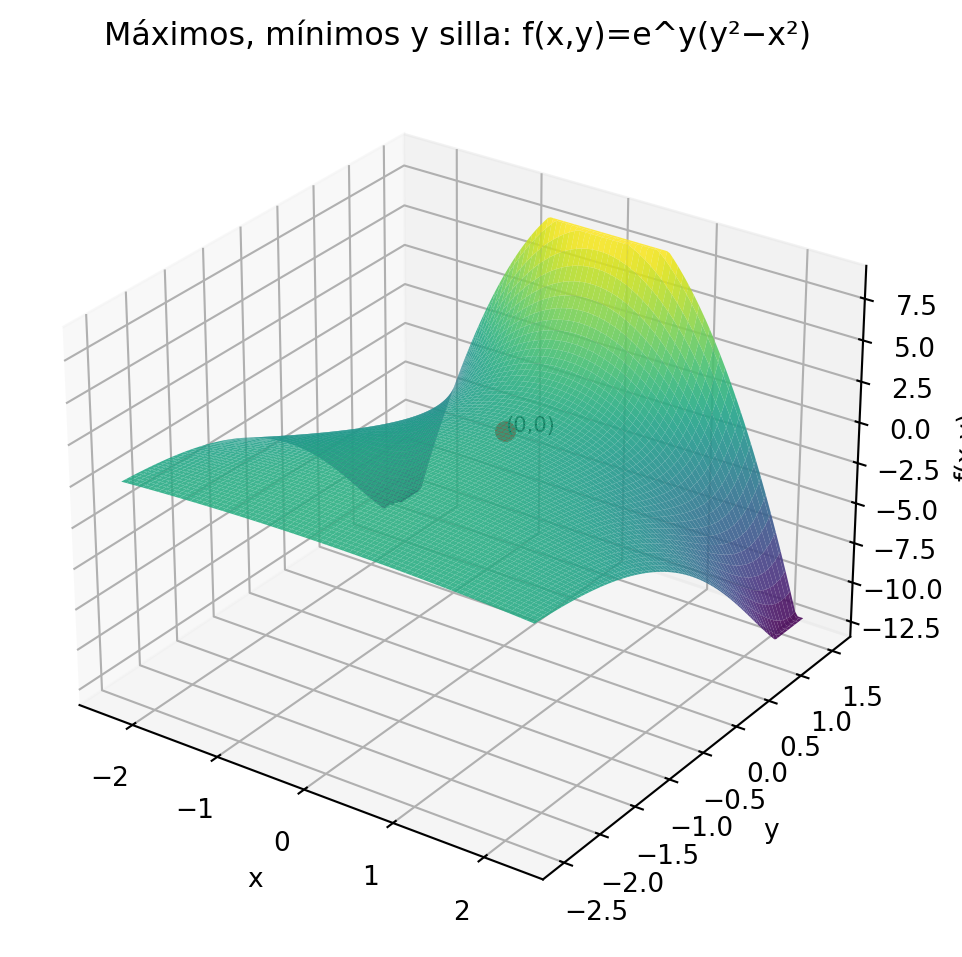
\includegraphics[width=0.82\textwidth]{graficas_taller_momento3/01_extremos_a.png}
\caption{Superficie de $f(x,y)=e^y(y^2-x^2)$.}
\label{fig:extremos-a}
\end{figure}


\begin{figure}[H]
\centering
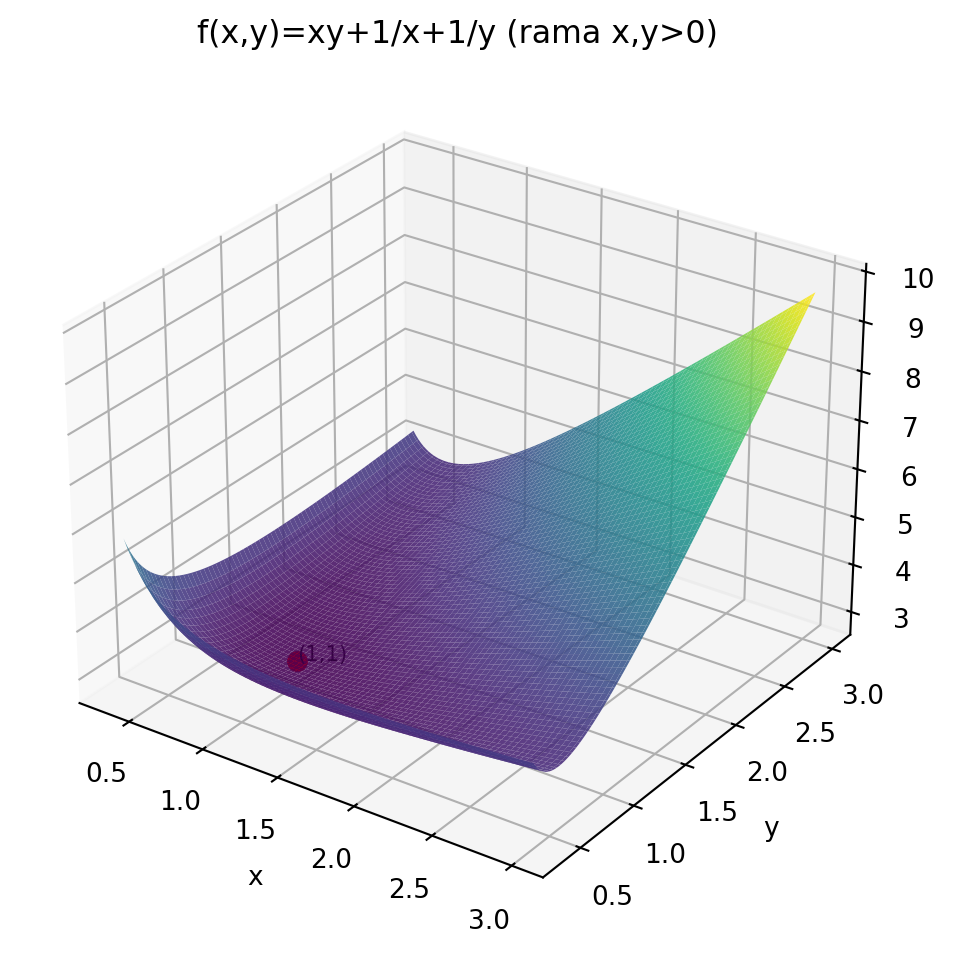
\includegraphics[width=0.82\textwidth]{graficas_taller_momento3/02_extremos_b.png}
\caption{Superficie de $f(x,y)=xy+1/x+1/y$ en la región $x,y>0$.}
\label{fig:extremos-b}
\end{figure}


\begin{figure}[H]
\centering
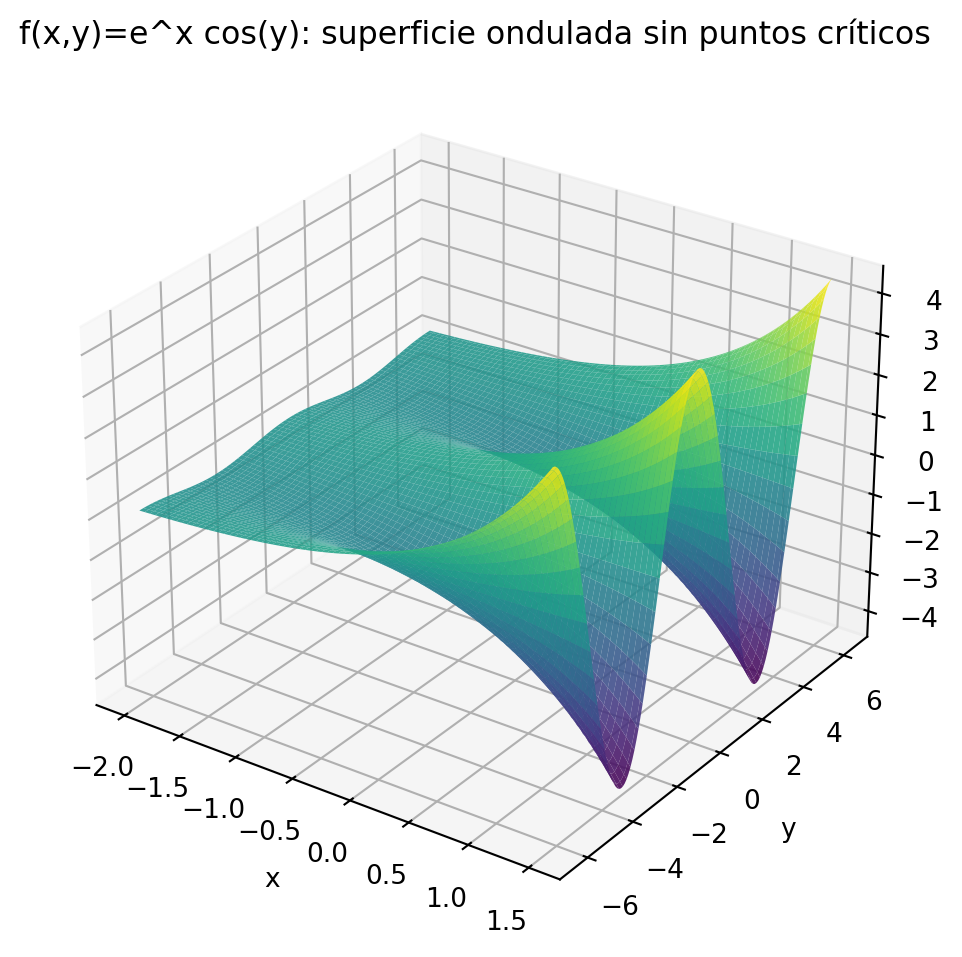
\includegraphics[width=0.82\textwidth]{graficas_taller_momento3/03_extremos_c.png}
\caption{Superficie de $f(x,y)=e^x\cos y$.}
\label{fig:extremos-c}
\end{figure}


\begin{figure}[H]
\centering
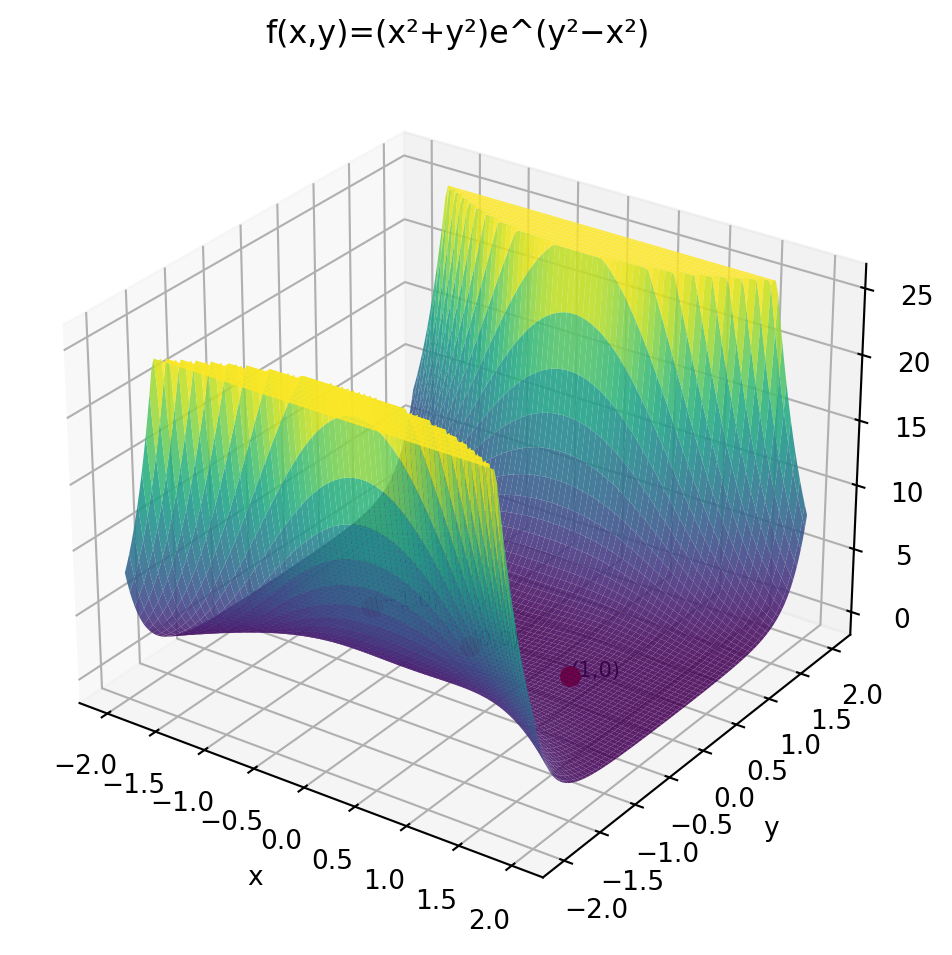
\includegraphics[width=0.82\textwidth]{graficas_taller_momento3/04_extremos_d.png}
\caption{Superficie de $f(x,y)=(x^2+y^2)e^{y^2-x^2}$.}
\label{fig:extremos-d}
\end{figure}


\begin{figure}[H]
\centering
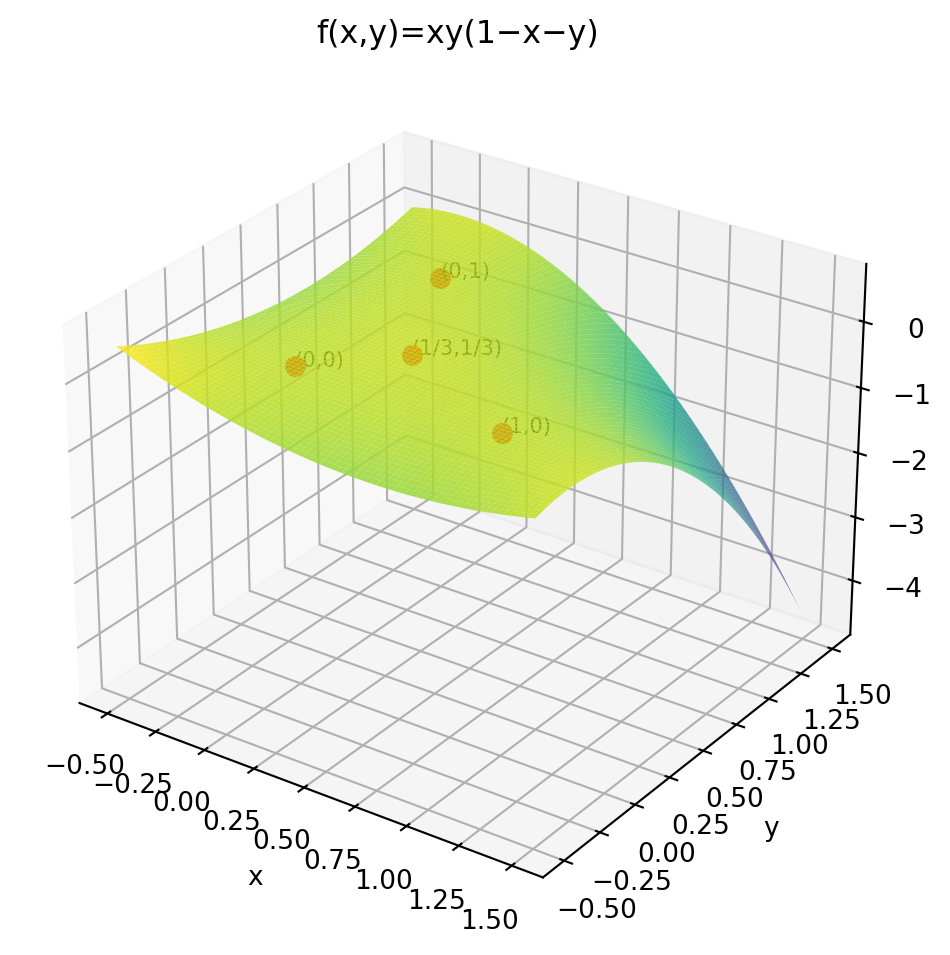
\includegraphics[width=0.82\textwidth]{graficas_taller_momento3/05_extremos_e.png}
\caption{Superficie de $f(x,y)=xy(1-x-y)$.}
\label{fig:extremos-e}
\end{figure}


\begin{figure}[H]
\centering
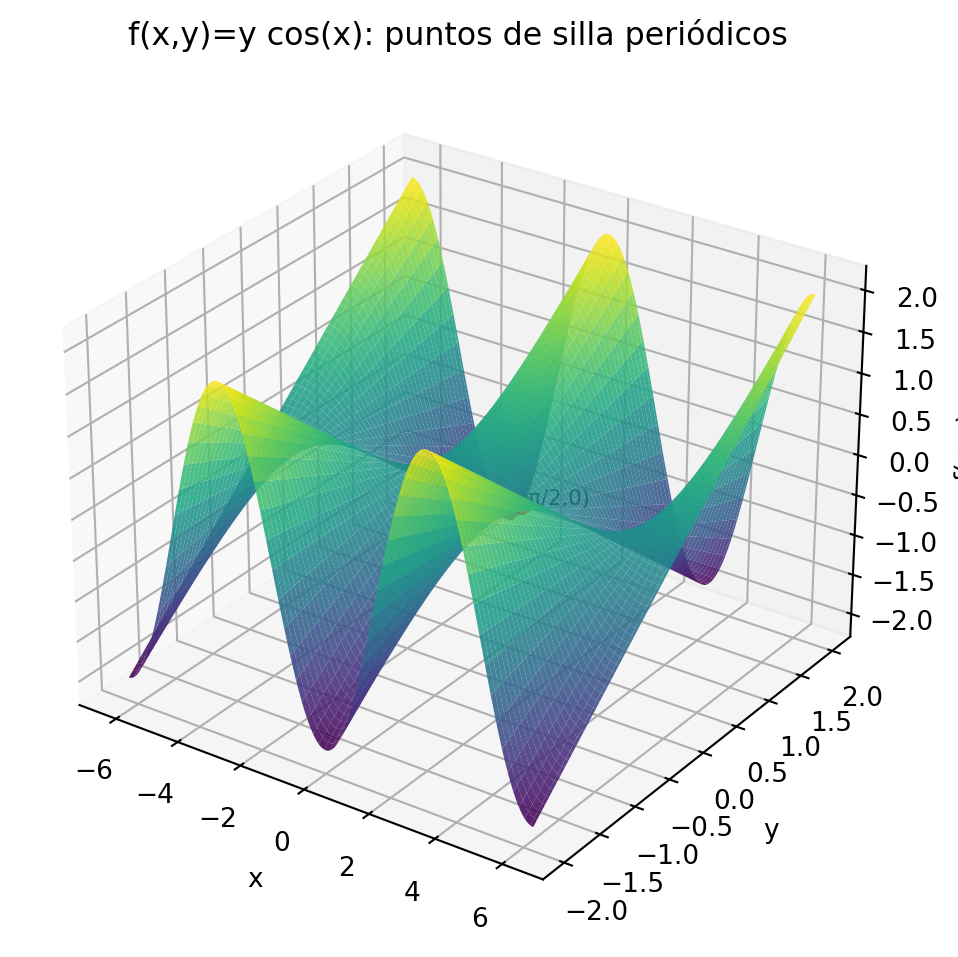
\includegraphics[width=0.82\textwidth]{graficas_taller_momento3/06_extremos_f.png}
\caption{Superficie de $f(x,y)=y\cos x$.}
\label{fig:extremos-f}
\end{figure}

\end{solution}

\chapter{Multiplicador de Lagrange}
\section*{Ejercicios}
\begin{exercise}
Utilizando multiplicadores de Lagrange, encuentre los valores máximo y minimo de la función sujeta
a la restricción o las restricciones dadas.
\begin{multicols}{2}
	(a)$f(x,y) = x^2+y^2 ; xy=1$\\
	\\
	(b) $f(x,y) = e^{xy} ; x^3+y^3=16$ \\
	\\
	(c) $f(x,y)= 3x + y; x^2+y^2 = 10 $\\
	\\
	(d) $f(x,y)= xyz; x^2 + 2y^3 + 3y^2 = 6$
 
\end{multicols}
\end{exercise}
\begin{solution}
\begin{enumerate}
	\item [a)] Para la función: $f(x, y) = x^2 + y^2$\\
Con la restricción de: $g(x, y) = xy = 1$\\
\\
Como primer paso, calculamos los gradientes
$$\nabla f = \left( \frac{\partial f}{\partial x}, \frac{\partial f}{\partial y} \right) = (2x, 2y)$$
$$\nabla g = \left( \frac{\partial g}{\partial x}, \frac{\partial g}{\partial y} \right) = (y, x)$$
 Como segundo paso, planteamos el sistema de ecuaciones
$$\begin{aligned}
2x &= \lambda y \quad &\text{(1)} \\
2y &= \lambda x \quad &\text{(2)} \\
xy &= 1 \quad &\text{(3)}
\end{aligned}$$
Como $xy = 1$, ni $x$ ni $y$ pueden ser cero ($x \neq 0, y \neq 0$).\\
\\
Resolvemos  el sistema:\\
\\
Multiplicamos la ecuación (1) por $x$ y la ecuación (2) por $y$:
$$2x^2 = \lambda xy$$
$$2y^2 = \lambda xy$$
Igualando ambas expresiones:
$$2x^2 = 2y^2 \implies x^2 = y^2 \implies y = \pm x$$
Sustituimos en la restricción $xy = 1$:


Si $y = x$:
$$x(x) = 1 \implies x^2 = 1 \implies x = \pm 1$$
Obtenemos los puntos críticos: $(1, 1)$ y $(-1, -1)$.


Si $y = -x$:
$$x(-x) = 1 \implies -x^2 = 1 \implies x^2 = -1 \quad \text{(no tiene soluciones reales)}$$


Evaluamos los puntos
$$f(1, 1) = 1^2 + 1^2 = 2$$
$$f(-1, -1) = (-1)^2 + (-1)^2 = 2$$
Analizando la restricción $y = \frac{1}{x}$, a medida que $x \to \infty$, $f(x, y) = x^2 + \frac{1}{x^2} \to \infty$, por lo que la función no tiene un valor máximo global.

Valor mínimo: $2$, alcanzado en los puntos $(1, 1)$ y $(-1, -1)$.\\
\\
Valor máximo: No existe (la función crece indefinidamente a lo largo de la restricción).\\


\item [b)]
Para la función: $f(x, y) = e^{xy}$\\
Con la restricción: $g(x, y) = x^3 + y^3 = 16$\\
\\
Calculamos los gradientes
$$\nabla f = \left( y e^{xy}, x e^{xy} \right)$$
$$\nabla g = \left( 3x^2, 3y^2 \right)$$
Planteamos el sistema de ecuaciones
$$\begin{aligned}
y e^{xy} &= 3\lambda x^2 \quad &\text{(1)} \\
x e^{xy} &= 3\lambda y^2 \quad &\text{(2)} \\
x^3 + y^3 &= 16 \quad &\text{(3)}
\end{aligned}$$
3. Resolver el sistema
Dividiendo la ecuación (1) entre la ecuación (2) (notando que si $x=0$, entonces $y=0$, lo cual contradice $x^3+y^3=16$):
$$\frac{y e^{xy}}{x e^{xy}} = \frac{3\lambda x^2}{3\lambda y^2} \implies \frac{y}{x} = \frac{x^2}{y^2}$$
Multiplicando en cruz:
$$y^3 = x^3 \implies y = x$$
Sustituimos $y = x$ en la restricción (3):
$$x^3 + x^3 = 16 \implies 2x^3 = 16 \implies x^3 = 8 \implies x = 2$$
Por lo tanto, $y = 2$. El punto crítico es $(2, 2)$.
4. Evaluar el punto y analizar el comportamiento
$$f(2, 2) = e^{(2)(2)} = e^4$$
Para verificar la existencia de extremos absolutos, analizamos la curva $x^3 + y^3 = 16$, la cual no es acotada (permite que $x \to -\infty$ mientras $y \to +\infty$):


Si tomamos $x \to -\infty$, entonces $y = \sqrt[3]{16 - x^3} \to +\infty$.


En este caso, el producto $xy \to -\infty$, lo que implica que:
$$\lim_{x \to -\infty} e^{xy} = 0$$
Dado que $e^{xy} > 0$ para todos los reales, la función se aproxima a $0$ pero nunca lo alcanza, por lo que no tiene un mínimo absoluto.


En cambio, el valor más alto alcanzado en la curva es local y globalmente acotado superiormente por $e^4$.


Valor máximo: $e^4$, alcanzado en el punto $(2, 2)$.


Valor mínimo: No existe (el ínfimo es $0$).



Parte (c)
Función a optimizar: $f(x, y) = 3x + y$
Restricción: $g(x, y) = x^2 + y^2 = 10$
(Nota: La restricción representa una circunferencia centrada en el origen de radio $\sqrt{10}$, la cual es un conjunto cerrado y acotado, garantizando la existencia de máximo y mínimo absolutos).
1. Calcular los gradientes
$$\nabla f = (3, 1)$$
$$\nabla g = (2x, 2y)$$
2. Plantear el sistema de ecuaciones
$$\begin{aligned}
3 &= 2\lambda x \quad &\text{(1)} \\
1 &= 2\lambda y \quad &\text{(2)} \\
x^2 + y^2 &= 10 \quad &\text{(3)}
\end{aligned}$$
3. Resolver el sistema
De (1) y (2), vemos que $\lambda \neq 0$:
$$x = \frac{3}{2\lambda}, \quad y = \frac{1}{2\lambda}$$
De aquí se deduce que:
$$x = 3y$$
Sustituyendo en la restricción (3):
$$(3y)^2 + y^2 = 10 \implies 9y^2 + y^2 = 10 \implies 10y^2 = 10 \implies y^2 = 1$$
Por lo tanto:
$$y = \pm 1$$

Si $y = 1 \implies x = 3(1) = 3$. Punto: $(3, 1)$
Si $y = -1 \implies x = 3(-1) = -3$. Punto: $(-3, -1)$

4. Evaluar los puntos
$$f(3, 1) = 3(3) + 1 = 9 + 1 = 10$$
$$f(-3, -1) = 3(-3) + (-1) = -9 - 1 = -10$$

Valor máximo: $10$, alcanzado en el punto $(3, 1)$.
Valor mínimo: $-10$, alcanzado en el punto $(-3, -1)$.


Parte (d)
Función a optimizar: $f(x, y, z) = xyz$
Restricción: En el enunciado aparece escrita como $x^2 + 2y^2 + 3y^2 = 6$.
Nota: Si se trata de un elipsoide en tres variables donde la última variable es $z$, la ecuación corresponde a $x^2 + 2y^2 + 3z^2 = 6$. A continuación se resuelve considerando esta forma estándar del elipsoide tridimensional.
Restricción: $g(x, y, z) = x^2 + 2y^2 + 3z^2 = 6$
1. Calcular los gradientes
$$\nabla f = (yz, xz, xy)$$
$$\nabla g = (2x, 4y, 6z)$$
2. Plantear el sistema de ecuaciones
$$\begin{aligned}
yz &= 2\lambda x \quad &\text{(1)} \\
xz &= 4\lambda y \quad &\text{(2)} \\
xy &= 6\lambda z \quad &\text{(3)} \\
x^2 + 2y^2 + 3z^2 &= 6 \quad &\text{(4)}
\end{aligned}$$
3. Resolver el sistema
Multiplicamos la ecuación (1) por $x$, la (2) por $y$, y la (3) por $z$:
$$xyz = 2\lambda x^2$$
$$xyz = 4\lambda y^2$$
$$xyz = 6\lambda z^2$$
Igualando los términos:
$$2\lambda x^2 = 4\lambda y^2 = 6\lambda z^2$$


Caso 1: $\lambda = 0$
Si $\lambda = 0$, entonces $xyz = 0$, lo que implica que al menos una de las variables es $0$. En cualquier punto donde alguna variable sea $0$, el valor de la función es:
$$f(x, y, z) = 0$$


Caso 2: $\lambda \neq 0$ (ninguna variable es cero)
Dividiendo entre $2\lambda$:
$$x^2 = 2y^2 = 3z^2$$
Sustituyendo estas relaciones en la restricción $x^2 + 2y^2 + 3z^2 = 6$:
$$x^2 + x^2 + x^2 = 6 \implies 3x^2 = 6 \implies x^2 = 2 \implies x = \pm \sqrt{2}$$
A partir de $x^2 = 2$:
$$2y^2 = 2 \implies y^2 = 1 \implies y = \pm 1$$
$$3z^2 = 2 \implies z^2 = \frac{2}{3} \implies z = \pm \sqrt{\frac{2}{3}} = \pm \frac{\sqrt{6}}{3}$$


4. Evaluar los puntos
El valor absoluto del producto en estos puntos es:
$$|f(x, y, z)| = |x| |y| |z| = (\sqrt{2})(1)\left(\sqrt{\frac{2}{3}}\right) = \sqrt{\frac{4}{3}} = \frac{2}{\sqrt{3}} = \frac{2\sqrt{3}}{3}$$
Dependiendo de los signos elegidos para $x, y, z$:


Si hay un número par de signos negativos (o ninguno), el producto es positivo:
$$f(x, y, z) = \frac{2\sqrt{3}}{3}$$


Si hay un número impar de signos negativos, el producto es negativo:
$$f(x, y, z) = -\frac{2\sqrt{3}}{3}$$


Valor máximo: $\dfrac{2\sqrt{3}}{3}$


Valor mínimo: $-\dfrac{2\sqrt{3}}{3}$



\end{enumerate}

% ===== Gráficas incorporadas =====


\begin{figure}[H]
\centering
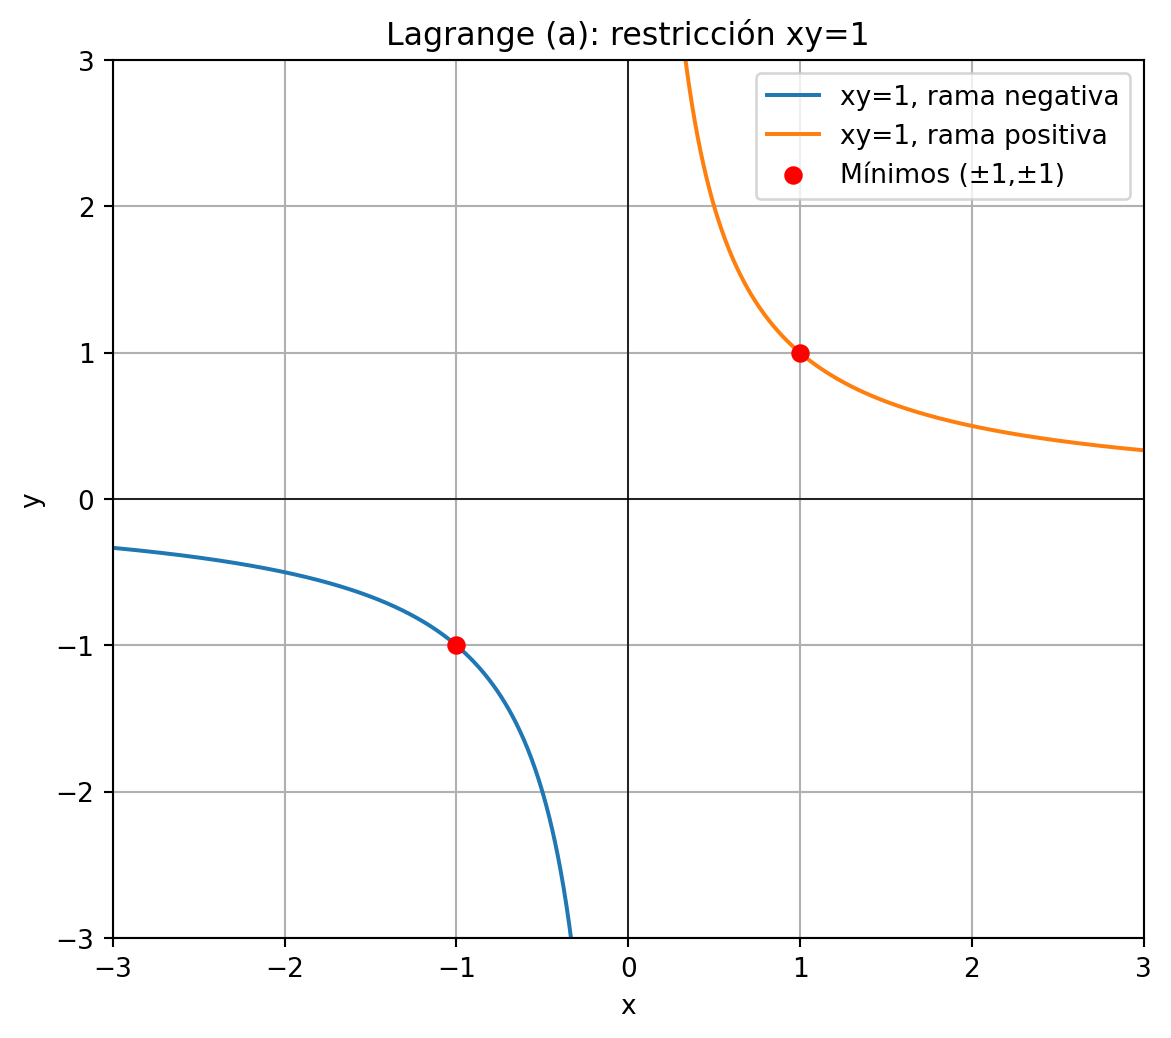
\includegraphics[width=0.82\textwidth]{graficas_taller_momento3/07_lagrange_a_xy1.png}
\caption{Curva de restricción $xy=1$ del inciso (a).}
\label{fig:lagrange-a}
\end{figure}


\begin{figure}[H]
\centering
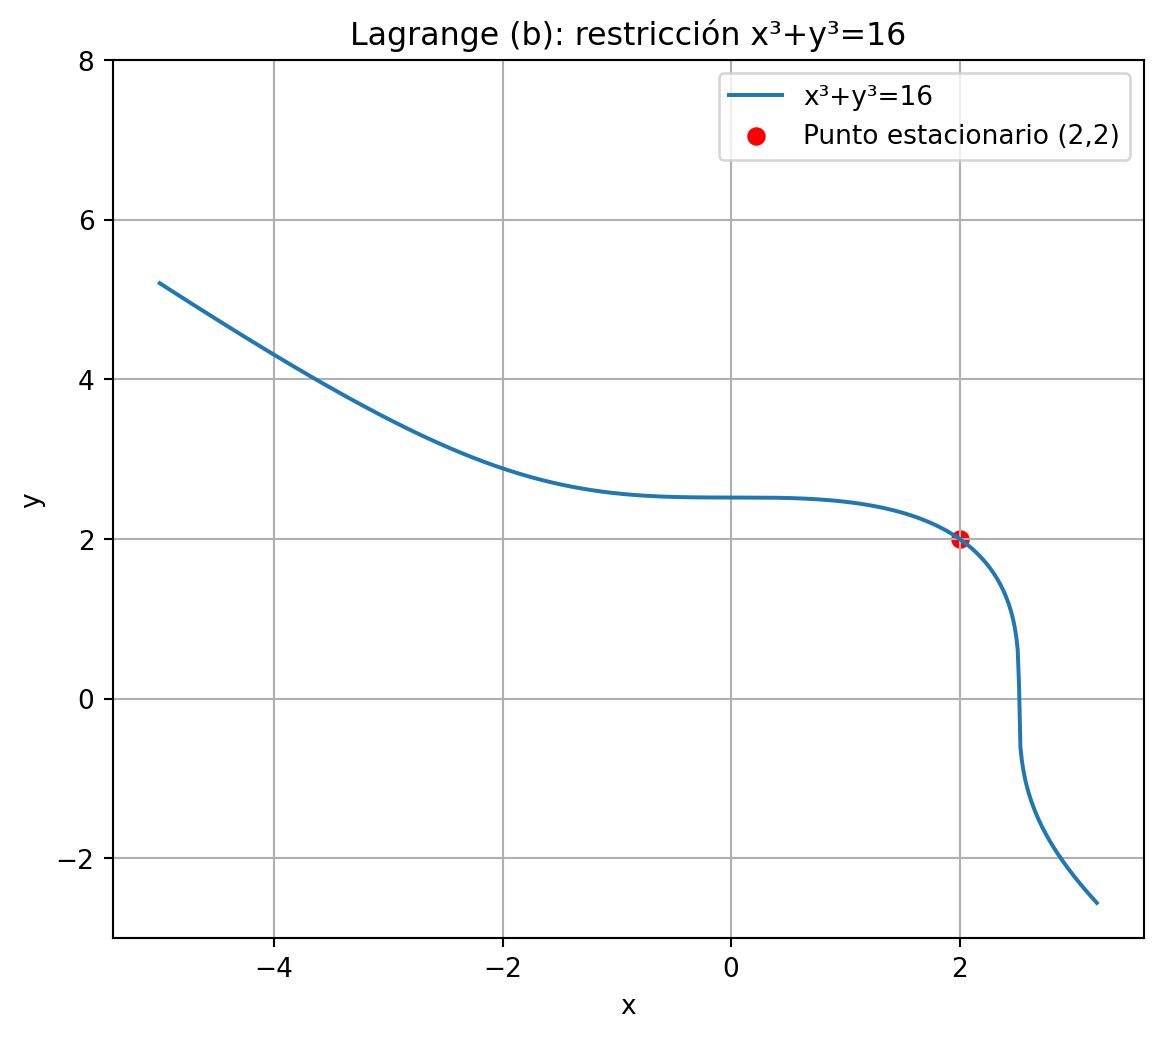
\includegraphics[width=0.82\textwidth]{graficas_taller_momento3/08_lagrange_b_constraint.png}
\caption{Curva de restricción $x^3+y^3=16$ del inciso (b).}
\label{fig:lagrange-b}
\end{figure}


\begin{figure}[H]
\centering
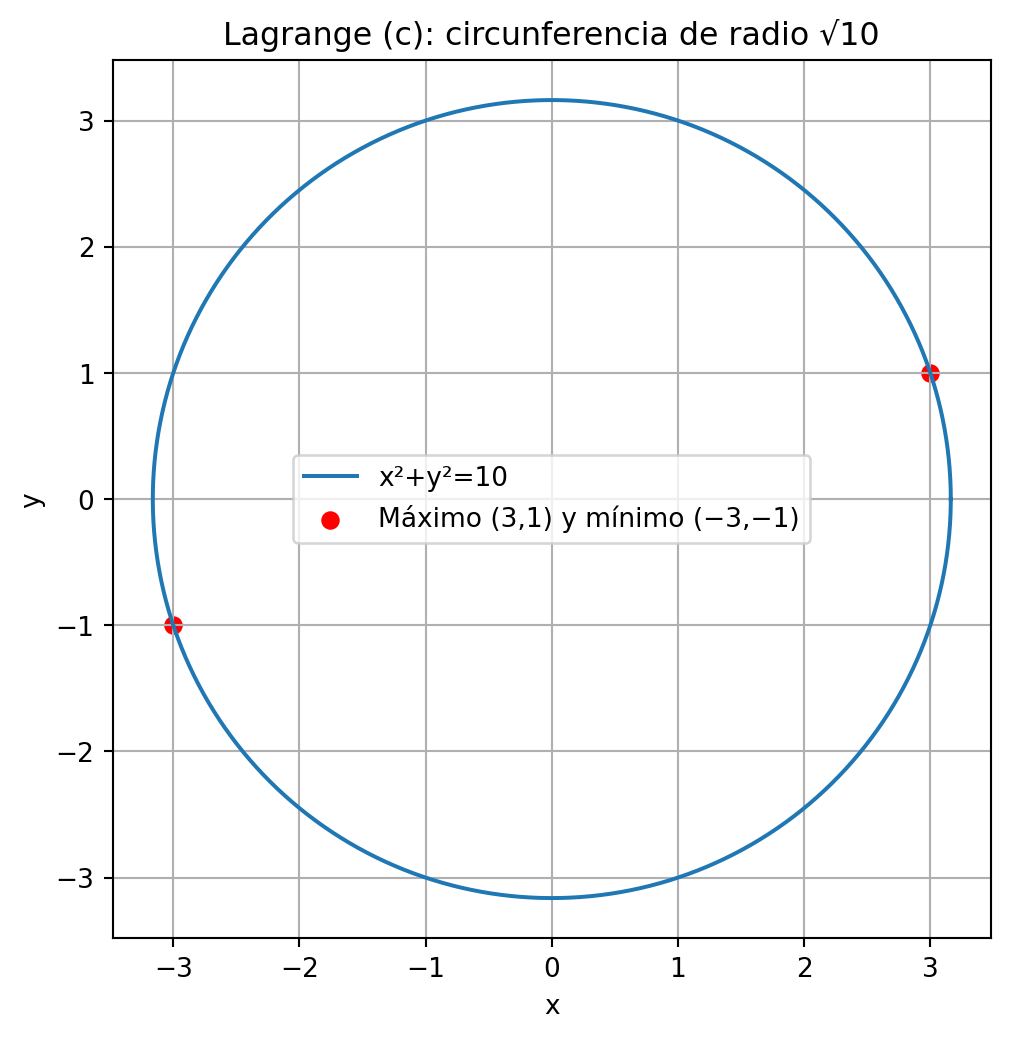
\includegraphics[width=0.82\textwidth]{graficas_taller_momento3/09_lagrange_c_circle.png}
\caption{Circunferencia de restricción $x^2+y^2=10$ del inciso (c).}
\label{fig:lagrange-c}
\end{figure}


\begin{figure}[H]
\centering
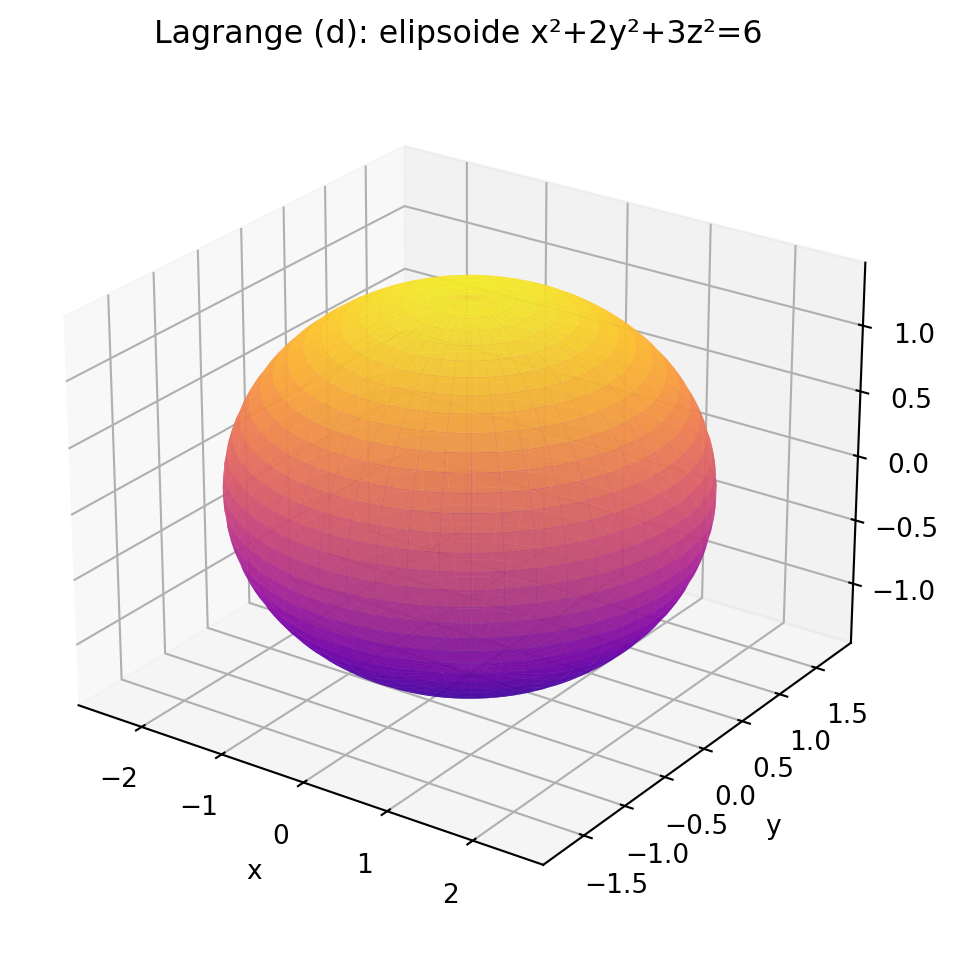
\includegraphics[width=0.82\textwidth]{graficas_taller_momento3/10_lagrange_d_ellipsoid.png}
\caption{Elipsoide de restricción $x^2+2y^2+3z^2=6$ usado en el inciso (d).}
\label{fig:lagrange-d}
\end{figure}

\end{solution}

\chapter{Iteracion de integrales}
\section*{Ejercicios}
\begin{exercise}
	Calcule la integral iterada
	\begin{multicols}{2}
	(a)	$\int_{0}^{1} \int_{0}^{1} y(x+y^2)^4  \,dxdy  $\\
	\\
	(b)	$\int_{0}^{1} \int_{0}^{3} e^{x+3y} \,dxdy$\\
	\\
	(c)	$\int_{1}^{3} \int_{1}^{5} \frac{\ln y}{xy} \,dydx$\\
     \\
	 (c)$\int_{0}^{1} \int_{0}^{1} xy\sqrt{x^2+y^2} \,dydx$\\

	\end{multicols}
\end{exercise}

\begin{solution}
A continuación se presenta la solución detallada de cada una de las integrales iteradas.



 Parte (a)

$$\int_{0}^{1} \int_{0}^{1} y(x + y^2)^4 \, dx \, dy$$

1. Integral interna (con respecto a $x$)
Tratamos a $y$ como una constante. La integral interna es:
$$\int_{0}^{1} y(x + y^2)^4 \, dx = y \int_{0}^{1} (x + y^2)^4 \, dx$$

Integrando respecto a $x$:
$$\int (x + y^2)^4 \, dx = \frac{(x + y^2)^5}{5}$$

Evaluamos entre los límites $x = 0$ y $x = 1$:
$$\left[ \frac{(x + y^2)^5}{5} \right]_{0}^{1} = \frac{(1 + y^2)^5 - (0 + y^2)^5}{5} = \frac{(1 + y^2)^5 - y^{10}}{5}$$

Por lo tanto, la expresión interna multiplicada por $y$ es:
$$\frac{1}{5} y (1 + y^2)^5 - \frac{1}{5} y^{11}$$

 2. Integral externa (con respecto a $y$)
$$\int_{0}^{1} \left( \frac{1}{5} y (1 + y^2)^5 - \frac{1}{5} y^{11} \right) dy = \frac{1}{5} \int_{0}^{1} y (1 + y^2)^5 \, dy - \frac{1}{5} \int_{0}^{1} y^{11} \, dy$$

 Para la primera parte, usamos la sustitución $u = 1 + y^2$, de donde $du = 2y \, dy \implies y \, dy = \frac{du}{2}$.  
  Los límites cambian: si $y = 0 \implies u = 1$; si $y = 1 \implies u = 2$:
  $$\int_{0}^{1} y(1 + y^2)^5 \, dy = \int_{1}^{2} u^5 \, \frac{du}{2} = \frac{1}{2} \left[ \frac{u^6}{6} \right]_{1}^{2} = \frac{2^6 - 1^6}{12} = \frac{64 - 1}{12} = \frac{63}{12} = \frac{21}{4}$$

*Para la segunda parte:
  $$\int_{0}^{1} y^{11} \, dy = \left[ \frac{y^{12}}{12} \right]_{0}^{1} = \frac{1}{12}$$

Combinamos ambos resultados:
$$\frac{1}{5} \left( \frac{21}{4} \right) - \frac{1}{5} \left( \frac{1}{12} \right) = \frac{1}{5} \left( \frac{63}{12} - \frac{1}{12} \right) = \frac{1}{5} \left( \frac{62}{12} \right) = \frac{1}{5} \left( \frac{31}{6} \right) = \frac{31}{30}$$

**Respuesta (a):**
$$\frac{31}{30}$$



 Parte (b)

$$\int_{0}^{1} \int_{0}^{3} e^{x+3y} \, dx \, dy$$

 1. Separar la integral
Aplicamos propiedades de los exponentes: $e^{x+3y} = e^x \cdot e^{3y}$.  
Como los límites de integración son constantes e independientes, la integral doble se puede separar en el producto de dos integrales simples:
$$\int_{0}^{1} \int_{0}^{3} e^x e^{3y} \, dx \, dy = \left( \int_{0}^{3} e^x \, dx \right) \left( \int_{0}^{1} e^{3y} \, dy \right)$$

 2. Calcular cada integral
 Integral respecto a $x$:
  $$\int_{0}^{3} e^x \, dx = \left[ e^x \right]_{0}^{3} = e^3 - e^0 = e^3 - 1$$

  Integral respecto a $y$:
  $$\int_{0}^{1} e^{3y} \, dy = \left[ \frac{e^{3y}}{3} \right]_{0}^{1} = \frac{e^{3(1)} - e^{3(0)}}{3} = \frac{e^3 - 1}{3}$$

 3. Multiplicar los resultados
$$\left( e^3 - 1 \right) \left( \frac{e^3 - 1}{3} \right) = \frac{(e^3 - 1)^2}{3}$$

Respuesta (b):
$$\frac{(e^3 - 1)^2}{3}$$

---

 Parte (c)

$$\int_{1}^{3} \int_{1}^{5} \frac{\ln y}{xy} \, dy \, dx$$

 1. Separar la integral
Reescribimos la función integrando separando las variables:
$$\frac{\ln y}{xy} = \left( \frac{1}{x} \right) \left( \frac{\ln y}{y} \right)$$

Al tener límites de integración constantes, separamos en el producto de dos integrales:
$$\int_{1}^{3} \frac{1}{x} \, dx \cdot \int_{1}^{5} \frac{\ln y}{y} \, dy$$

 2. Calcular cada integral
 Integral respecto a $x$:
  $$\int_{1}^{3} \frac{1}{x} \, dx = \left[ \ln|x| \right]_{1}^{3} = \ln 3 - \ln 1 = \ln 3$$

 Integral respecto a $y$:
  Usamos sustitución simple con $u = \ln y$, de modo que $du = \frac{1}{y} \, dy$.  
  Los límites cambian: si $y = 1 \implies u = \ln 1 = 0$; si $y = 5 \implies u = \ln 5$:
  $$\int_{1}^{5} \frac{\ln y}{y} \, dy = \int_{0}^{\ln 5} u \, du = \left[ \frac{u^2}{2} \right]_{0}^{\ln 5} = \frac{(\ln 5)^2}{2}$$

 3. Multiplicar los resultados
$$\ln 3 \cdot \frac{(\ln 5)^2}{2} = \frac{1}{2} (\ln 3)(\ln 5)^2$$

Respuesta (c):
$$\frac{1}{2} (\ln 3)(\ln 5)^2$$

---

 Parte (d)

$$\int_{0}^{1} \int_{0}^{1} xy\sqrt{x^2 + y^2} \, dy \, dx$$

 1. Integral interna (con respecto a $y$)
Tratamos a $x$ como una constante:
$$\int_{0}^{1} xy\sqrt{x^2 + y^2} \, dy = x \int_{0}^{1} y(x^2 + y^2)^{1/2} \, dy$$

Realizamos la sustitución $u = x^2 + y^2$, de donde $du = 2y \, dy \implies y \, dy = \frac{du}{2}$.  
Límites para $u$:
 Cuando $y = 0 \implies u = x^2$
 Cuando $y = 1 \implies u = x^2 + 1$

Integrando:
$$x \int_{x^2}^{x^2 + 1} u^{1/2} \frac{du}{2} = \frac{x}{2} \left[ \frac{u^{3/2}}{3/2} \right]_{x^2}^{x^2 + 1} = \frac{x}{3} \left[ (x^2 + 1)^{3/2} - (x^2)^{3/2} \right]$$

Como $x \ge 0$, tenemos $(x^2)^{3/2} = x^3$:
$$= \frac{1}{3} x(x^2 + 1)^{3/2} - \frac{1}{3} x^4$$

 2. Integral externa (con respecto a $x$)
$$\int_{0}^{1} \left( \frac{1}{3} x(x^2 + 1)^{3/2} - \frac{1}{3} x^4 \right) dx = \frac{1}{3} \int_{0}^{1} x(x^2 + 1)^{3/2} \, dx - \frac{1}{3} \int_{0}^{1} x^4 \, dx$$

 Para la primera parte, hacemos la sustitución $w = x^2 + 1$, con $dw = 2x \, dx \implies x \, dx = \frac{dw}{2}$.  
  Límites: si $x = 0 \implies w = 1$; si $x = 1 \implies w = 2$:
  $$\int_{0}^{1} x(x^2 + 1)^{3/2} \, dx = \int_{1}^{2} w^{3/2} \frac{dw}{2} = \frac{1}{2} \left[ \frac{w^{5/2}}{5/2} \right]_{1}^{2} = \frac{1}{5} \left[ 2^{5/2} - 1^{5/2} \right] = \frac{1}{5} (4\sqrt{2} - 1)$$

 Para la segunda parte:
  $$\int_{0}^{1} x^4 \, dx = \left[ \frac{x^5}{5} \right]_{0}^{1} = \frac{1}{5}$$

Sustituyendo ambos términos:
$$\frac{1}{3} \left( \frac{4\sqrt{2} - 1}{5} \right) - \frac{1}{3} \left( \frac{1}{5} \right) = \frac{4\sqrt{2} - 1 - 1}{15} = \frac{4\sqrt{2} - 2}{15}$$

**Respuesta (d):**
$$\frac{4\sqrt{2} - 2}{15} = \frac{2(2\sqrt{2} - 1)}{15}$$

% ===== Gráficas incorporadas =====


\begin{figure}[H]
\centering
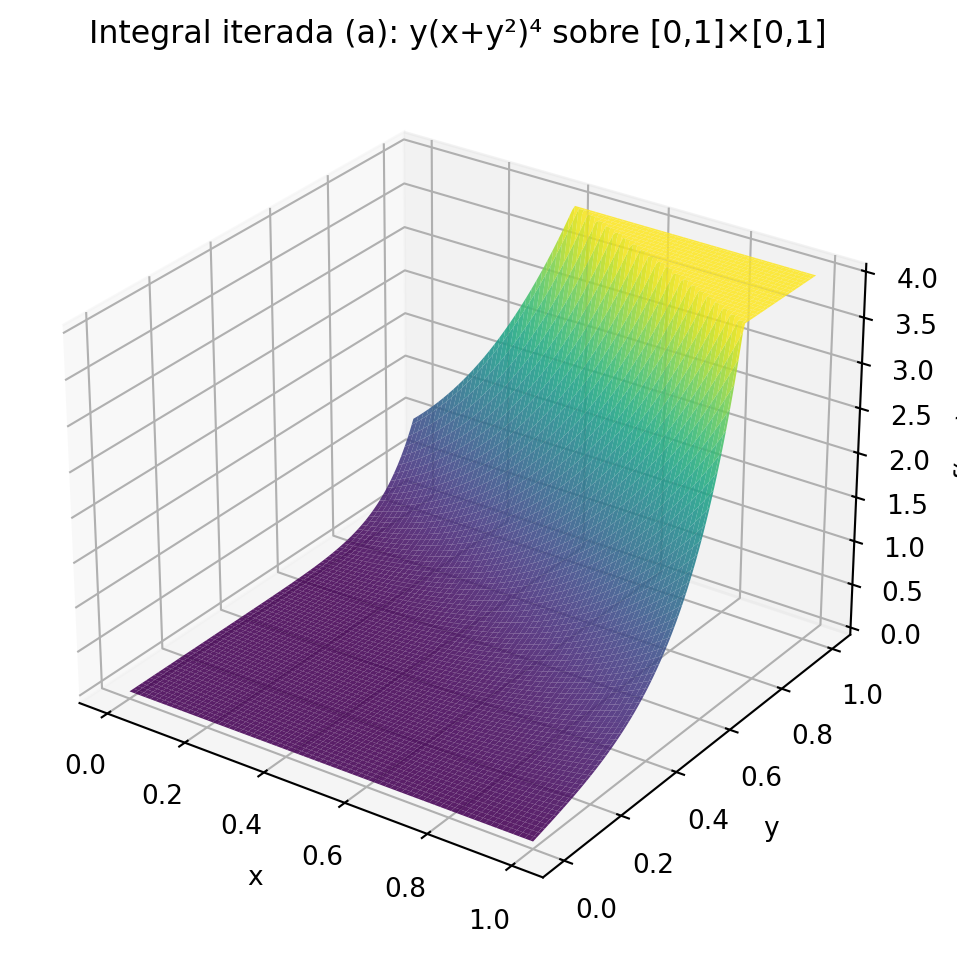
\includegraphics[width=0.82\textwidth]{graficas_taller_momento3/11_iterada_a.png}
\caption{Superficie del integrando $y(x+y^2)^4$ en $[0,1]\times[0,1]$.}
\label{fig:iterada-a}
\end{figure}


\begin{figure}[H]
\centering
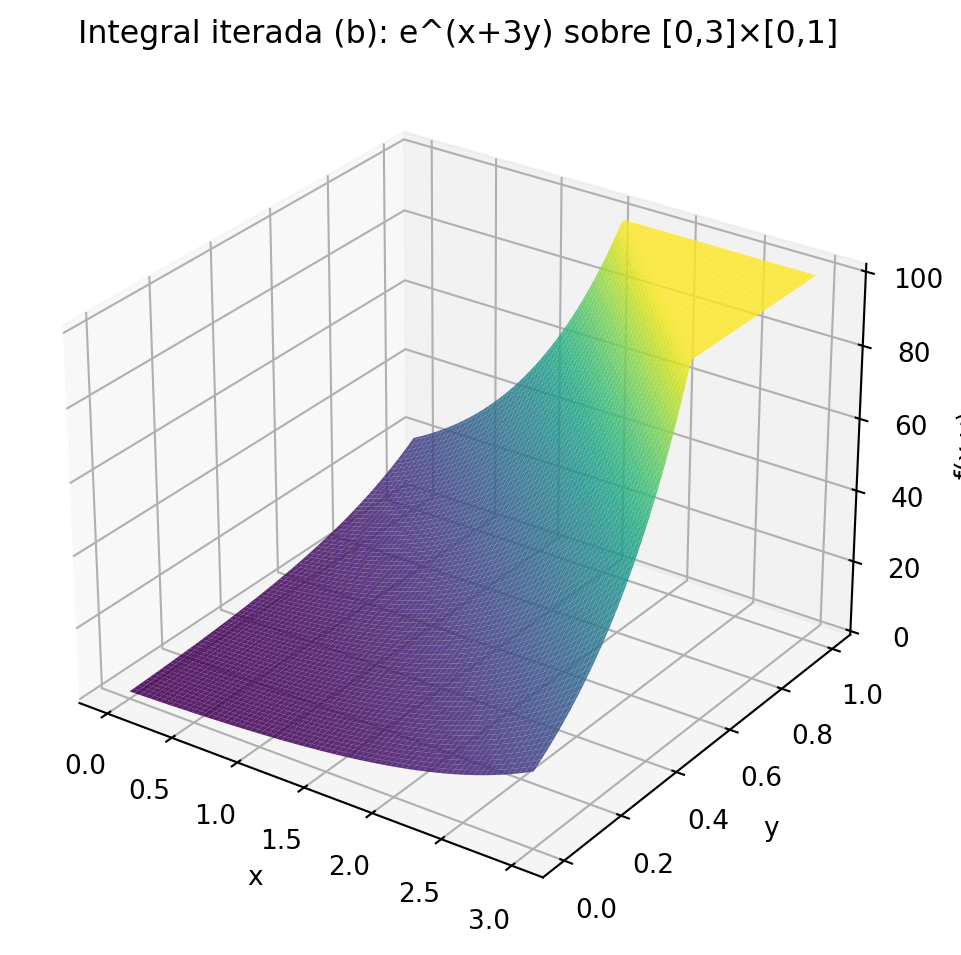
\includegraphics[width=0.82\textwidth]{graficas_taller_momento3/12_iterada_b.png}
\caption{Superficie del integrando $e^{x+3y}$ en $[0,3]\times[0,1]$.}
\label{fig:iterada-b}
\end{figure}


\begin{figure}[H]
\centering
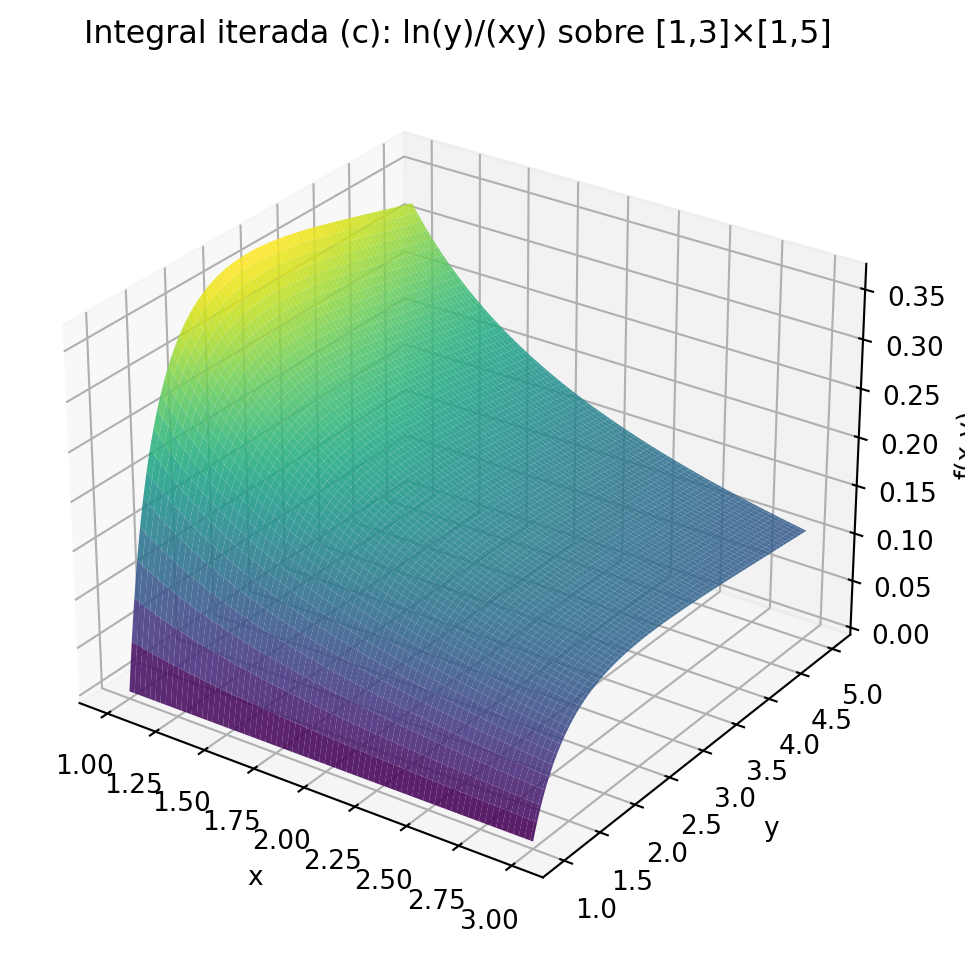
\includegraphics[width=0.82\textwidth]{graficas_taller_momento3/13_iterada_c.png}
\caption{Superficie del integrando $\ln(y)/(xy)$ en $[1,3]\times[1,5]$.}
\label{fig:iterada-c}
\end{figure}


\begin{figure}[H]
\centering
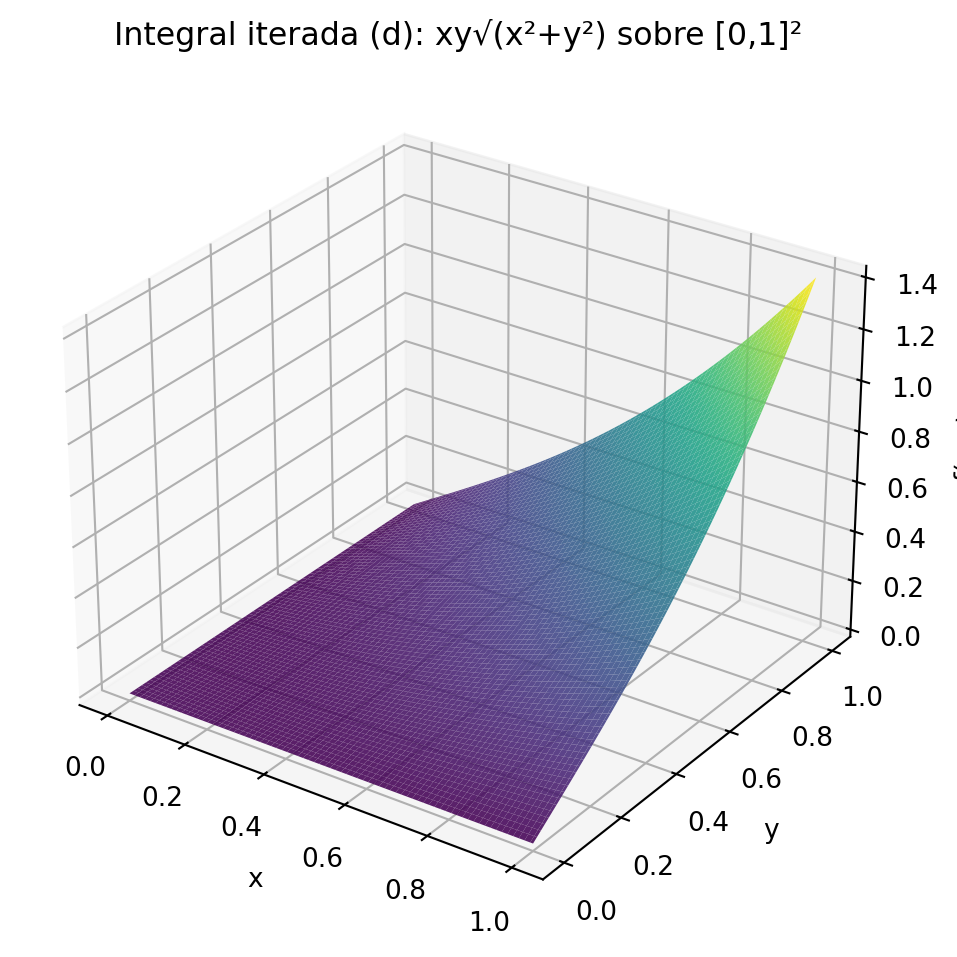
\includegraphics[width=0.82\textwidth]{graficas_taller_momento3/14_iterada_d.png}
\caption{Superficie del integrando $xy\sqrt{x^2+y^2}$ en $[0,1]\times[0,1]$.}
\label{fig:iterada-d}
\end{figure}

\end{solution}

\chapter{Integrales dobles}
\section*{Ejercicios}
\begin{exercise}
	Calcule la integral doble.
\begin{enumerate}
    \item[a)] $\displaystyle \iint_{R} \sin(x + y) \, dA, \quad R = \left\{(x, y) \mid 0 \le x \le \frac{\pi}{2}, \, 0 \le y \le \frac{\pi}{2}\right\}$
    \item[b)] $\displaystyle \iint_{R} \frac{xy^2}{x^2 + 1} \, dA, \quad R = \left\{(x, y) \mid 0 \le x \le 2, \, 1 \le y \le 2\right\}$
    \item[c)] $\displaystyle \iint_{R} \frac{1}{x + y + z} \, dA, \quad R = [1, 3] \times [1, 2]$
\end{enumerate}
\end{exercise}

\begin{solution}
Para resolver cada una de estas integrales dobles sobre regiones rectangulares, aplicamos el **Teorema de Fubini**, el cual nos permite transformar la integral doble en integrales iteradas sencillas.

---

 Inciso (a)

Calcular:
$$\iint_{R} \sin(x + y) \, dA, \quad R = \left\{(x, y) \;\middle|\; 0 \le x \le \frac{\pi}{2}, \, 0 \le y \le \frac{\pi}{2}\right\}$$

 Paso 1: Plantear la integral iterada
Escribimos la integral con los límites dados:
$$\int_{0}^{\pi/2} \int_{0}^{\pi/2} \sin(x + y) \, dy \, dx$$

 Paso 2: Resolver la integral interna con respecto a $y$
Tratamos a $x$ como una constante. La antiderivada de $\sin(x + y)$ respecto a $y$ es $-\cos(x + y)$:
$$\int_{0}^{\pi/2} \sin(x + y) \, dy = \Big[ -\cos(x + y) \Big]_{y=0}^{y=\pi/2}$$

Evaluamos en los límites superior e inferior:
$$= -\cos\left(x + \frac{\pi}{2}\right) - \big(-\cos(x + 0)\big)$$
$$= -\cos\left(x + \frac{\pi}{2}\right) + \cos(x)$$

Usando la identidad trigonométrica $\cos\left(x + \frac{\pi}{2}\right) = -\sin(x)$:
$$= -(-\sin(x)) + \cos(x) = \sin(x) + \cos(x)$$

 Paso 3: Resolver la integral externa con respecto a $x$
Ahora integramos el resultado respecto a $x$:
$$\int_{0}^{\pi/2} \big(\sin(x) + \cos(x)\big) \, dx = \Big[ -\cos(x) + \sin(x) \Big]_{0}^{\pi/2}$$

Evaluamos en los límites:
- En $x = \frac{\pi}{2}$:
  $$-\cos\left(\frac{\pi}{2}\right) + \sin\left(\frac{\pi}{2}\right) = -0 + 1 = 1$$

- En $x = 0$:
  $$-\cos(0) + \sin(0) = -1 + 0 = -1$$

Restamos el límite inferior del superior:
$$1 - (-1) = 1 + 1 = 2$$

Respuesta (a):
$$\iint_{R} \sin(x + y) \, dA = 2$$



 Inciso (b)

Calcular:
$$\iint_{R} \frac{xy^2}{x^2 + 1} \, dA, \quad R = \big\{(x, y) \;\big|\; 0 \le x \le 2, \, 1 \le y \le 2\big\}$$

Paso 1: Separar las variables
Notemos que la función se puede factorizar como el producto de una función que solo depende de $x$ y otra que solo depende de $y$:
$$f(x, y) = \left(\frac{x}{x^2 + 1}\right) \cdot y^2$$

Como los límites de integración son constantes, podemos separar la integral doble en el producto de dos integrales simples:
$$\iint_{R} \frac{xy^2}{x^2 + 1} \, dA = \left(\int_{0}^{2} \frac{x}{x^2 + 1} \, dx\right) \cdot \left(\int_{1}^{2} y^2 \, dy\right)$$

 Paso 2: Resolver la integral en $x$
$$\int_{0}^{2} \frac{x}{x^2 + 1} \, dx$$

Aplicamos el método de sustitución:
- Sea $u = x^2 + 1 \implies du = 2x \, dx \implies x \, dx = \frac{du}{2}$
- Nuevos límites:
  - Si $x = 0 \implies u = 0^2 + 1 = 1$
  - Si $x = 2 \implies u = 2^2 + 1 = 5$

Sustituyendo:
$$\int_{1}^{5} \frac{1}{u} \cdot \frac{du}{2} = \frac{1}{2} \Big[ \ln|u| \Big]_{1}^{5} = \frac{1}{2} \big(\ln(5) - \ln(1)\big)$$

Como $\ln(1) = 0$:
$$= \frac{1}{2} \ln(5)$$

 Paso 3: Resolver la integral en $y$
$$\int_{1}^{2} y^2 \, dy = \left[ \frac{y^3}{3} \right]_{1}^{2} = \frac{2^3}{3} - \frac{1^3}{3} = \frac{8}{3} - \frac{1}{3} = \frac{7}{3}$$

 Paso 4: Multiplicar ambos resultados
$$\iint_{R} \frac{xy^2}{x^2 + 1} \, dA = \left(\frac{1}{2} \ln(5)\right) \cdot \left(\frac{7}{3}\right) = \frac{7}{6} \ln(5)$$

Respuesta (b):
$$\iint_{R} \frac{xy^2}{x^2 + 1} \, dA = \frac{7}{6} \ln(5)$$



Inciso (c)

Calcular:
$$\iint_{R} \frac{1}{x + y + z} \, dA, \quad R = [1, 3] \times [1, 2]$$

(Nota: En esta integral doble sobre las variables $x$ e $y$, la variable $z$ actúa como un parámetro constante, con $1 \le x \le 3$ y $1 \le y \le 2$).

 Paso 1: Plantear la integral iterada
$$\int_{1}^{2} \int_{1}^{3} \frac{1}{x + y + z} \, dx \, dy$$

 Paso 2: Resolver la integral interna con respecto a $x$
Como $y$ y $z$ son constantes con respecto a $x$:
$$\int_{1}^{3} \frac{1}{x + (y + z)} \, dx = \Big[ \ln(x + y + z) \Big]_{x=1}^{x=3}$$

Evaluamos en los límites:
$$= \ln(3 + y + z) - \ln(1 + y + z)$$

 Paso 3: Resolver la integral externa con respecto a $y$
$$\int_{1}^{2} \Big( \ln(y + z + 3) - \ln(y + z + 1) \Big) \, dy$$

Recordemos la fórmula de integración para el logaritmo natural:
$$\int \ln(u) \, du = u \ln(u) - u$$

Por lo tanto:
$$\int \ln(y + c) \, dy = (y + c)\ln(y + c) - (y + c)$$

Aplicamos esto a cada término:

1. Para $\int_{1}^{2} \ln(y + z + 3) \, dy$:
   $$\Big[ (y + z + 3)\ln(y + z + 3) - (y + z + 3) \Big]_{1}^{2}$$
   - En $y = 2$:
     $$(z + 5)\ln(z + 5) - (z + 5)$$
   - En $y = 1$:
     $$(z + 4)\ln(z + 4) - (z + 4)$$
   - Restando:
     $$(z + 5)\ln(z + 5) - (z + 4)\ln(z + 4) - 1$$

2. Para $\int_{1}^{2} \ln(y + z + 1) \, dy$:
   $$\Big[ (y + z + 1)\ln(y + z + 1) - (y + z + 1) \Big]_{1}^{2}$$
   - En $y = 2$:
     $$(z + 3)\ln(z + 3) - (z + 3)$$
   - En $y = 1$:
     $$(z + 2)\ln(z + 2) - (z + 2)$$
   - Restando:
     $$(z + 3)\ln(z + 3) - (z + 2)\ln(z + 2) - 1$$

Paso 4: Restar ambas integrales
Restamos la segunda expresión de la primera (notando que los términos $-1$ se cancelan):
$$\big[(z + 5)\ln(z + 5) - (z + 4)\ln(z + 4) - 1\big] - \big[(z + 3)\ln(z + 3) - (z + 2)\ln(z + 2) - 1\big]$$

$$= (z + 5)\ln(z + 5) - (z + 4)\ln(z + 4) - (z + 3)\ln(z + 3) + (z + 2)\ln(z + 2)$$

(En caso de que se trate de un error tipográfico del texto y la variable fuera $z = 0$, el resultado numérico se obtiene evaluando en $z = 0$: $5\ln(5) - 4\ln(4) - 3\ln(3) + 2\ln(2)$).

Respuesta (c):
$$\iint_{R} \frac{1}{x + y + z} \, dA = (z + 5)\ln(z + 5) - (z + 4)\ln(z + 4) - (z + 3)\ln(z + 3) + (z + 2)\ln(z + 2)$$

% ===== Gráficas incorporadas =====


\begin{figure}[H]
\centering
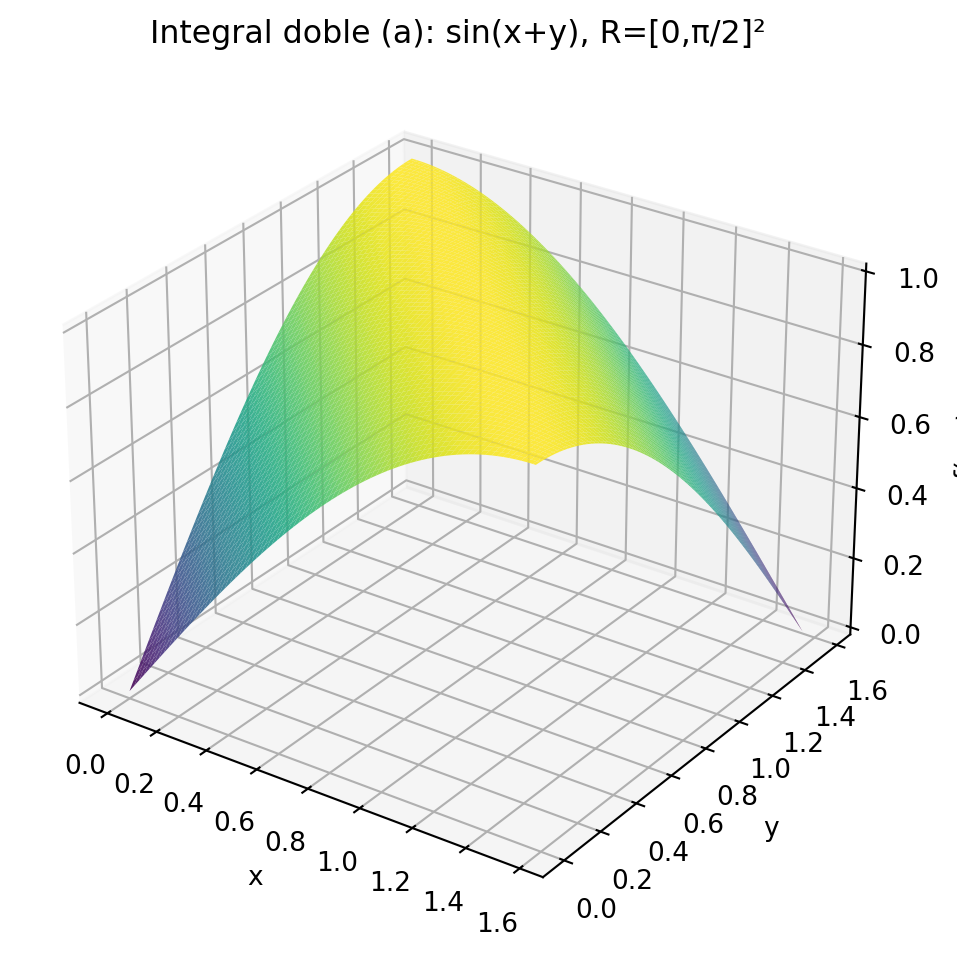
\includegraphics[width=0.82\textwidth]{graficas_taller_momento3/15_doble_a.png}
\caption{Superficie de $\sin(x+y)$ sobre la región rectangular del inciso (a).}
\label{fig:doble-a}
\end{figure}


\begin{figure}[H]
\centering
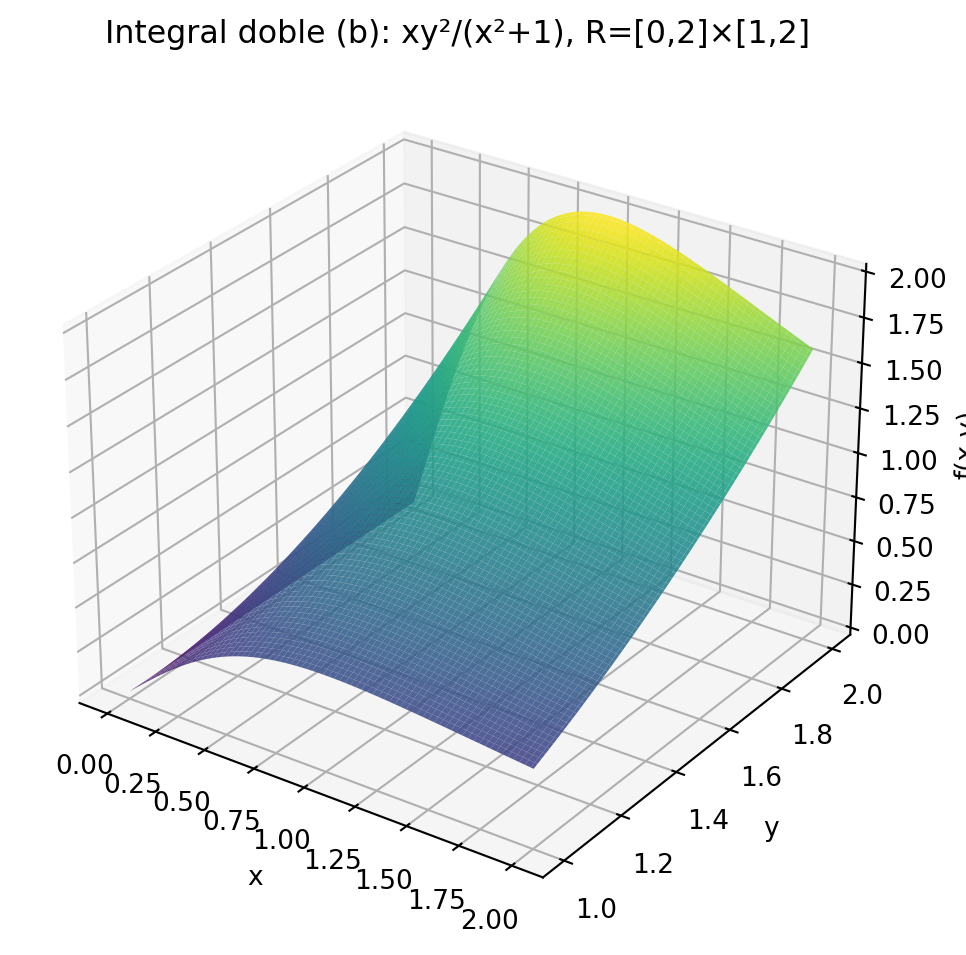
\includegraphics[width=0.82\textwidth]{graficas_taller_momento3/16_doble_b.png}
\caption{Superficie de $xy^2/(x^2+1)$ sobre la región rectangular del inciso (b).}
\label{fig:doble-b}
\end{figure}


\begin{figure}[H]
\centering
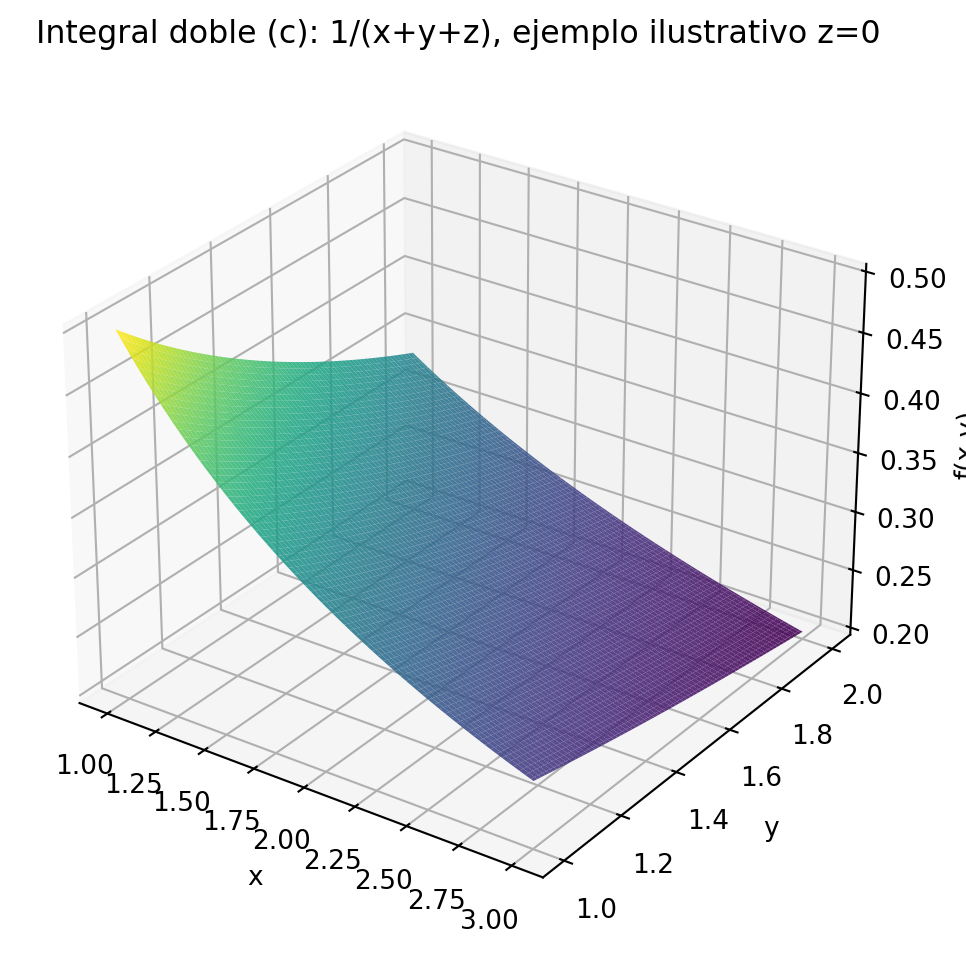
\includegraphics[width=0.82\textwidth]{graficas_taller_momento3/17_doble_c.png}
\caption{Superficie ilustrativa de $1/(x+y+z)$ tomando $z=0$ para visualizarla.}
\label{fig:doble-c}
\end{figure}

\end{solution}

\chapter{Aplicaciones de la integral}
\section*{Ejercicios}
\begin{exercise}
	Sea $E$ el sólido que está en el primer octante acotado por las superficies $4y^2 + z = 9$, $3x + y = 12$, $x = 0$, $y = 0$, $z = 0$. Expresar sin resolver
\[
\iiint_{E} xyz \, dV
\]
de 4 formas distintas en coordenadas cartesianas con 2 órdenes de integración diferentes.
\end{exercise}


\begin{solution}

	Para resolver este problema, primero debemos entender y describir geométricamente la región sólida $E$ en el primer octante, para luego plantear las integrales iteradas correspondientes.

---

 Análisis del sólido $E$

El sólido $E$ se encuentra en el **primer octante**, lo que significa que:
$$x \ge 0, \quad y \ge 0, \quad z \ge 0$$

Las superficies que lo delimitan son:
1. Cilindro parabólico:** $4y^2 + z = 9 \implies z = 9 - 4y^2$.
2. Plano:** $3x + y = 12 \implies x = \frac{12 - y}{3} = 4 - \frac{y}{3}$ (o de forma equivalente $y = 12 - 3x$).
3. Planos coordenados:** $x = 0$, $y = 0$, $z = 0$.

 1. Rango de las variables

 Para $z$: Dado que $z \ge 0$ y $z = 9 - 4y^2$, el valor mínimo es $z = 0$ y el máximo ocurre cuando $y = 0$, es decir, $z \in [0, 9]$.
 Para $y$:
  De la condición $z \ge 0$, tenemos:
    $$9 - 4y^2 \ge 0 \implies 4y^2 \le 9 \implies y^2 \le \frac{9}{4} \implies 0 \le y \le \frac{3}{2}$$
   Por otro lado, la recta $3x + y = 12$ interseca el eje $y$ en $y = 12$. Sin embargo, la cota más restrictiva impuesta por el cilindro parabólico con $z \ge 0$ es $y \le \frac{3}{2}$.
   Como $\frac{3}{2} < 12$, la variable $y$ varía únicamente en el intervalo:
    $$y \in \left[0, \frac{3}{2}\right]$$
 Para $x$:
   Para cualquier valor de $y \in \left[0, \frac{3}{2}\right]$, la variable $x$ varía desde el plano $x = 0$ hasta el plano inclinado:
    $$x = \frac{12 - y}{3} = 4 - \frac{y}{3}$$
   Cuando $y = 0$, $x = 4$.
   Cuando $y = \frac{3}{2}$, $x = 4 - \frac{1}{2} = \frac{7}{2}$.



 Planteamiento de las integrales

El enunciado solicita expresar la integral triple:
$$\iiint_E x\,y\,z\,dV$$
de **4 formas distintas** usando **órdenes de integración diferentes**. Existen en total 6 órdenes posibles en coordenadas cartesianas ($dz\,dx\,dy$, $dz\,dy\,dx$, $dx\,dz\,dy$, $dx\,dy\,dz$, $dy\,dz\,dx$, $dy\,dx\,dz$). A continuación se desarrollan 4 de las formas más claras y directas:


 Forma 1: Orden $dz\,dx\,dy$

Proyectamos el sólido sobre el plano $xy$:
 La región en el plano $xy$ se puede describir dejando $y$ como variable exterior:
  $$0 \le y \le \frac{3}{2}$$
 Para cada $y$ fijo, $x$ va desde el eje $y$ ($x = 0$) hasta la recta:
  $$0 \le x \le \frac{12 - y}{3}$$
 Para cada punto $(x, y)$, la altura $z$ va desde el plano $xy$ ($z = 0$) hasta el paraboloide:
  $$0 \le z \le 9 - 4y^2$$

La integral queda:
$$\int_{0}^{3/2} \int_{0}^{\frac{12 - y}{3}} \int_{0}^{9 - 4y^2} x\,y\,z\,dz\,dx\,dy$$



 Forma 2: Orden $dx\,dz\,dy$

Manteniendo la proyección sobre el plano $yz$:
 En el plano $yz$, la región está delimitada por los ejes coordenados y la parábola $z = 9 - 4y^2$:
  $$0 \le y \le \frac{3}{2}$$
  $$0 \le z \le 9 - 4y^2$$
 Para cualquier $(y, z)$, el sólido está acotado en $x$ desde el plano $x = 0$ hasta el plano $x = \frac{12 - y}{3}$:
  $$0 \le x \le \frac{12 - y}{3}$$

La integral queda:
$$\int_{0}^{3/2} \int_{0}^{9 - 4y^2} \int_{0}^{\frac{12 - y}{3}} x\,y\,z\,dx\,dz\,dy$$



 Forma 3: Orden $dx\,dy\,dz$

En el plano $yz$, también podemos integrar primero con respecto a $y$ y luego respecto a $z$:
 De $z = 9 - 4y^2$, despejamos $y \ge 0$:
  $$4y^2 = 9 - z \implies y = \frac{\sqrt{9 - z}}{2}$$
  Los límites para $z$ van desde $0$ hasta el vértice en $z = 9$:
  $$0 \le z \le 9$$
 Para cada $z$, la variable $y$ va desde $y = 0$ hasta la curva:
  $$0 \le y \le \frac{\sqrt{9 - z}}{2}$$
 Finalmente, para la variable $x$:
  $$0 \le x \le \frac{12 - y}{3}$$

La integral queda:
$$\int_{0}^{9} \int_{0}^{\frac{\sqrt{9 - z}}{2}} \int_{0}^{\frac{12 - y}{3}} x\,y\,z\,dx\,dy\,dz$$

---

 Forma 4: Orden $dz\,dy\,dx$

Si en el plano $xy$ integramos primero con respecto a $y$ y luego con respecto a $x$, observemos el rango de $x$:
 El valor mínimo de $x$ es $0$.
 El valor máximo ocurre cuando $y = 0$, que es $x = 4$.
 Sin embargo, la recta $y = 12 - 3x$ corta el valor límite superior $y = \frac{3}{2}$ en:
  $$\frac{3}{2} = 12 - 3x \implies 3x = \frac{21}{2} \implies x = \frac{7}{2}$$

Esto divide la región del plano $xy$ en dos subregiones:
1. Para $0 \le x \le \frac{7}{2}$: la variable $y$ va desde $0$ hasta $\frac{3}{2}$.
2. Para $\frac{7}{2} \le x \le 4$: la variable $y$ va desde $0$ hasta la recta $y = 12 - 3x$.

Por lo tanto, en este orden la integral se expresa como la suma de dos integrales:

$$\int_{0}^{7/2} \int_{0}^{3/2} \int_{0}^{9 - 4y^2} x\,y\,z\,dz\,dy\,dx \;+\; \int_{7/2}^{4} \int_{0}^{12 - 3x} \int_{0}^{9 - 4y^2} x\,y\,z\,dz\,dy\,dx$$


% ===== Gráficas incorporadas =====


\begin{figure}[H]
\centering
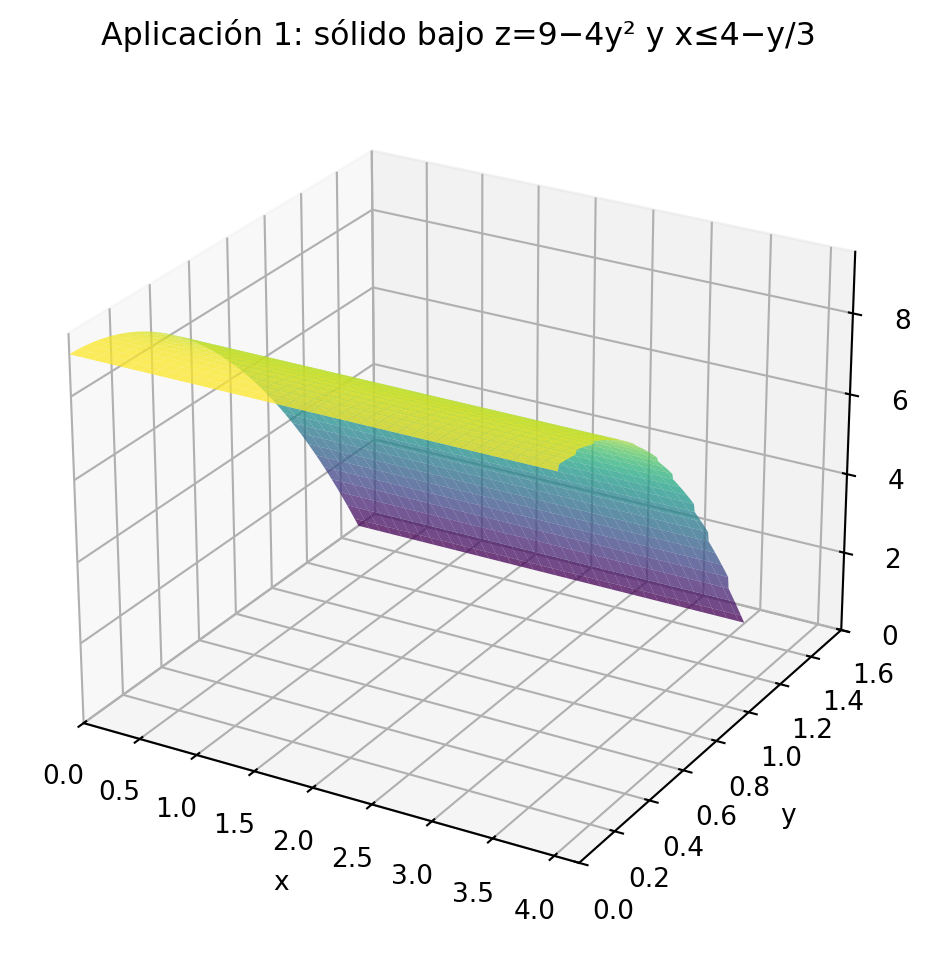
\includegraphics[width=0.82\textwidth]{graficas_taller_momento3/18_aplicacion_solid1.png}
\caption{Superficie superior del sólido del primer ejercicio de aplicaciones.}
\label{fig:aplicacion-solido-1}
\end{figure}


\begin{figure}[H]
\centering
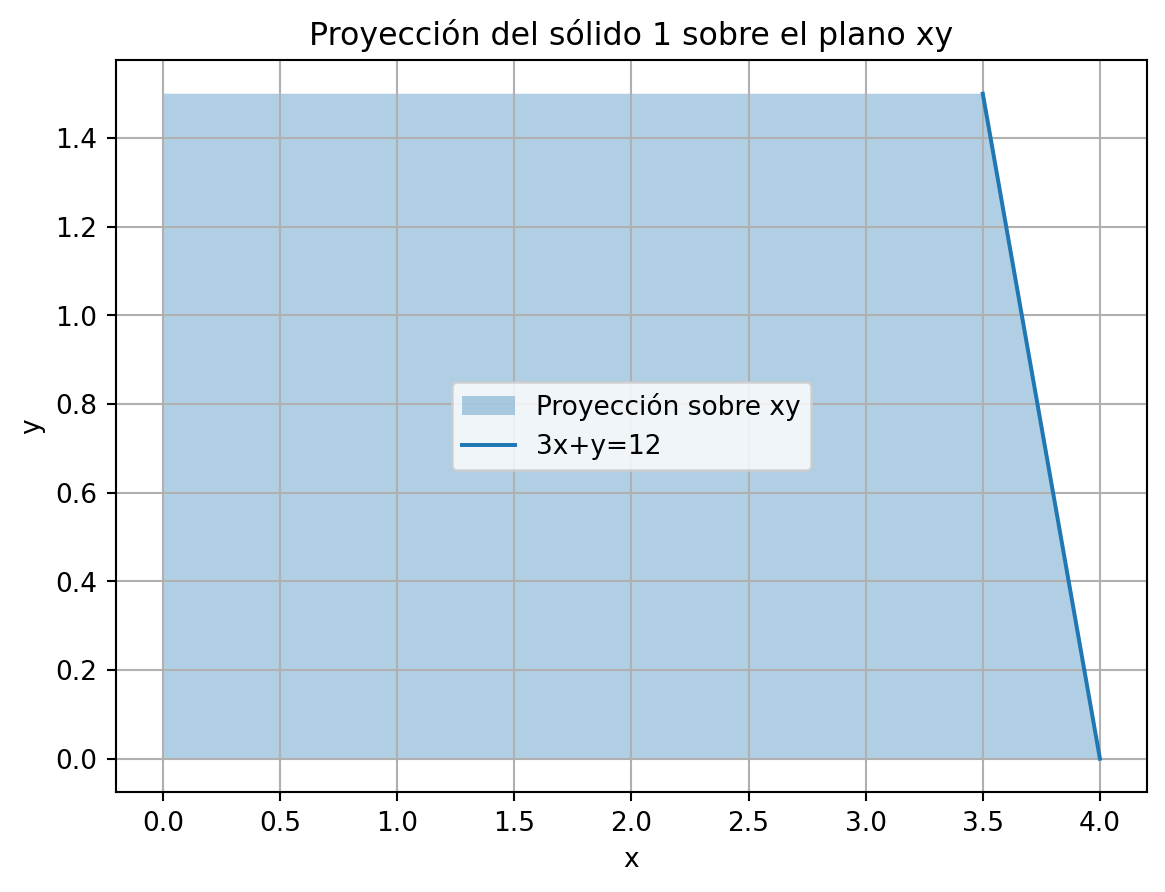
\includegraphics[width=0.82\textwidth]{graficas_taller_momento3/19_aplicacion_solid1_xy.png}
\caption{Proyección de la región del primer sólido sobre el plano $xy$.}
\label{fig:aplicacion-proyeccion-1}
\end{figure}

\end{solution}
\begin{exercise}
Sea $E$ el sólido por debajo del plano $2y + z = 12$, por encima del plano $z = 0$ y entre las superficies $y = 3x^2$ y $y = 4 - x^2$. Resolver
\[
\iiint_{E} x^2 \, dV
\]
\end{exercise}
\begin{solution}
Análisis y descripción del sólido $E$

El sólido $E$ está delimitado por las siguientes condiciones:
1. Límites en $z$:
    Por encima del plano: $z = 0$.
    Por debajo del plano: $2y + z = 12 \implies z = 12 - 2y$.
   *Por lo tanto:
     $$0 \le z \le 12 - 2y$$

2. Límites en el plano $xy$ (cilindros parabólicos):
    Las curvas que encierran la región en el plano $xy$ son $y = 3x^2$ e $y = 4 - x^2$.
    Hallamos los puntos de intersección igualando las expresiones de $y$:
     $$3x^2 = 4 - x^2 \implies 4x^2 = 4 \implies x^2 = 1 \implies x = \pm 1$$
    Para cualquier valor en el intervalo $[-1, 1]$, tenemos que $4 - x^2 \ge 3x^2$ (por ejemplo, en $x = 0$, $4 \ge 0$). Por lo tanto:
     $$-1 \le x \le 1$$
     $$3x^2 \le y \le 4 - x^2$$

(Nótese que en esta región $y \le 4$, por lo que $z = 12 - 2y \ge 12 - 2(4) = 4 > 0$, garantizando que el techo $z = 12 - 2y$ siempre está por encima de $z = 0$).

Planteamiento de la integral
La integral a resolver es:
$$\iiint_E x^2\,dV = \int_{-1}^{1} \int_{3x^2}^{4 - x^2} \int_{0}^{12 - 2y} x^2\,dz\,dy\,dx$$



 Paso 1: Integración con respecto a $z$

Integramos respecto a $z$ considerando a $x$ e $y$ como constantes:
$$\int_{0}^{12 - 2y} x^2\,dz = x^2 \Big[ z \Big]_{0}^{12 - 2y} = x^2(12 - 2y)$$



 Paso 2: Integración con respecto a $y$

Ahora integramos la expresión resultante con respecto a $y$:
$$\int_{3x^2}^{4 - x^2} x^2(12 - 2y)\,dy = x^2 \int_{3x^2}^{4 - x^2} (12 - 2y)\,dy$$

Calculamos la antiderivada con respecto a $y$:
$$\int (12 - 2y)\,dy = 12y - y^2$$

Evaluamos entre los límites $y = 3x^2$ y $y = 4 - x^2$:
$$\Big[ 12y - y^2 \Big]_{3x^2}^{4 - x^2} = \Big( 12(4 - x^2) - (4 - x^2)^2 \Big) - \Big( 12(3x^2) - (3x^2)^2 \Big)$$

Desarrollamos cada parte:
Límite superior:
  $$12(4 - x^2) - (16 - 8x^2 + x^4) = 48 - 12x^2 - 16 + 8x^2 - x^4 = 32 - 4x^2 - x^4$$

 Límite inferior:
  $$36x^2 - 9x^4$$

Restamos el límite inferior del superior:
$$(32 - 4x^2 - x^4) - (36x^2 - 9x^4) = 32 - 40x^2 + 8x^4 = 8(4 - 5x^2 + x^4)$$

Multiplicando por el factor $x^2$ exterior:
$$x^2(32 - 40x^2 + 8x^4) = 32x^2 - 40x^4 + 8x^6$$



 Paso 3: Integración con respecto a $x$

La integral respecto a $x$ queda:
$$\int_{-1}^{1} (32x^2 - 40x^4 + 8x^6)\,dx$$

Dado que la función integrando es **par** (todas las potencias de $x$ son pares), podemos aprovechar la simetría sobre el intervalo simétrico $[-1, 1]$:
$$\int_{-1}^{1} (32x^2 - 40x^4 + 8x^6)\,dx = 2 \int_{0}^{1} (32x^2 - 40x^4 + 8x^6)\,dx$$

Calculamos la antiderivada término a término:
$$\int (32x^2 - 40x^4 + 8x^6)\,dx = \frac{32}{3}x^3 - \frac{40}{5}x^5 + \frac{8}{7}x^7 = \frac{32}{3}x^3 - 8x^5 + \frac{8}{7}x^7$$

Evaluamos en los límites de $0$ a $1$:
$$\Big[ \frac{32}{3}x^3 - 8x^5 + \frac{8}{7}x^7 \Big]_0^1 = \frac{32}{3} - 8 + \frac{8}{7}$$

Operamos las fracciones con común denominador $21$:
$$\frac{32}{3} - 8 + \frac{8}{7} = \frac{32 \cdot 7 - 8 \cdot 21 + 8 \cdot 3}{21} = \frac{224 - 168 + 24}{21} = \frac{80}{21}$$

Multiplicamos por el factor $2$:
$$2 \cdot \frac{80}{21} = \frac{160}{21}$$


 Resultado final

$$\iiint_E x^2\,dV = \frac{160}{21}$$


% ===== Gráficas incorporadas =====


\begin{figure}[H]
\centering
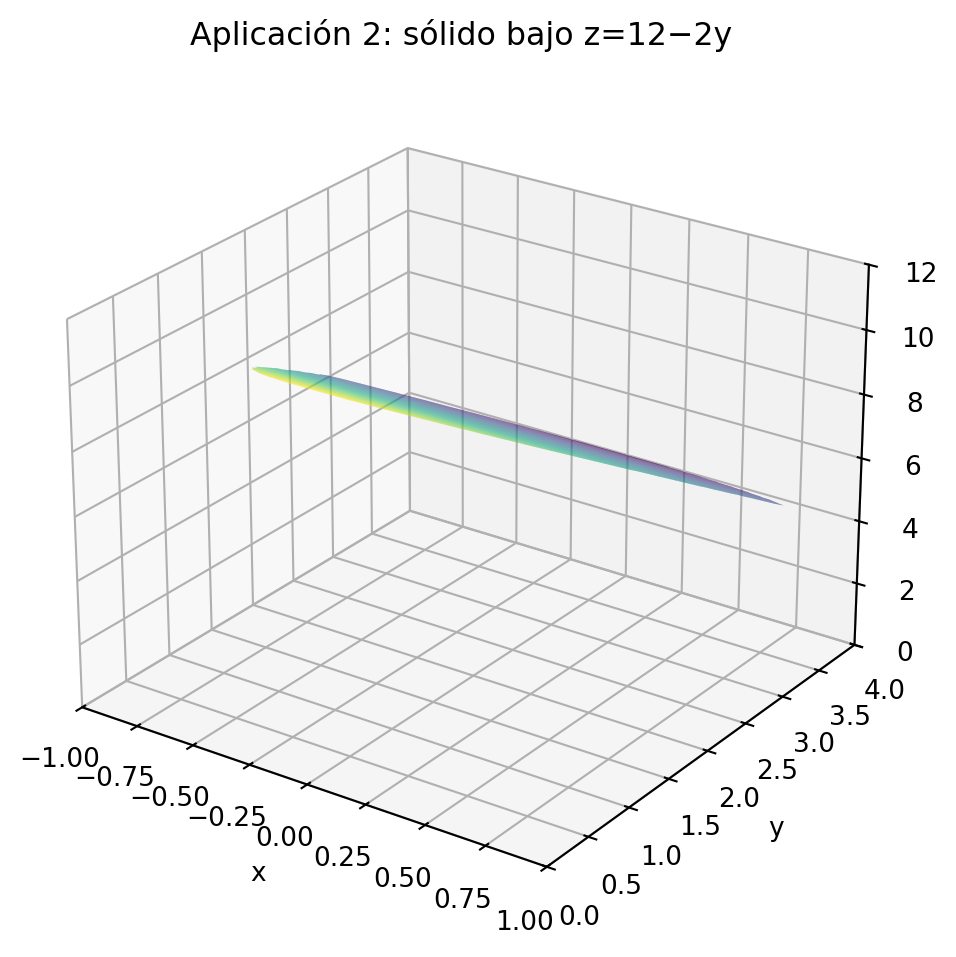
\includegraphics[width=0.82\textwidth]{graficas_taller_momento3/20_aplicacion_solid2.png}
\caption{Superficie superior del sólido del segundo ejercicio de aplicaciones.}
\label{fig:aplicacion-solido-2}
\end{figure}


\begin{figure}[H]
\centering
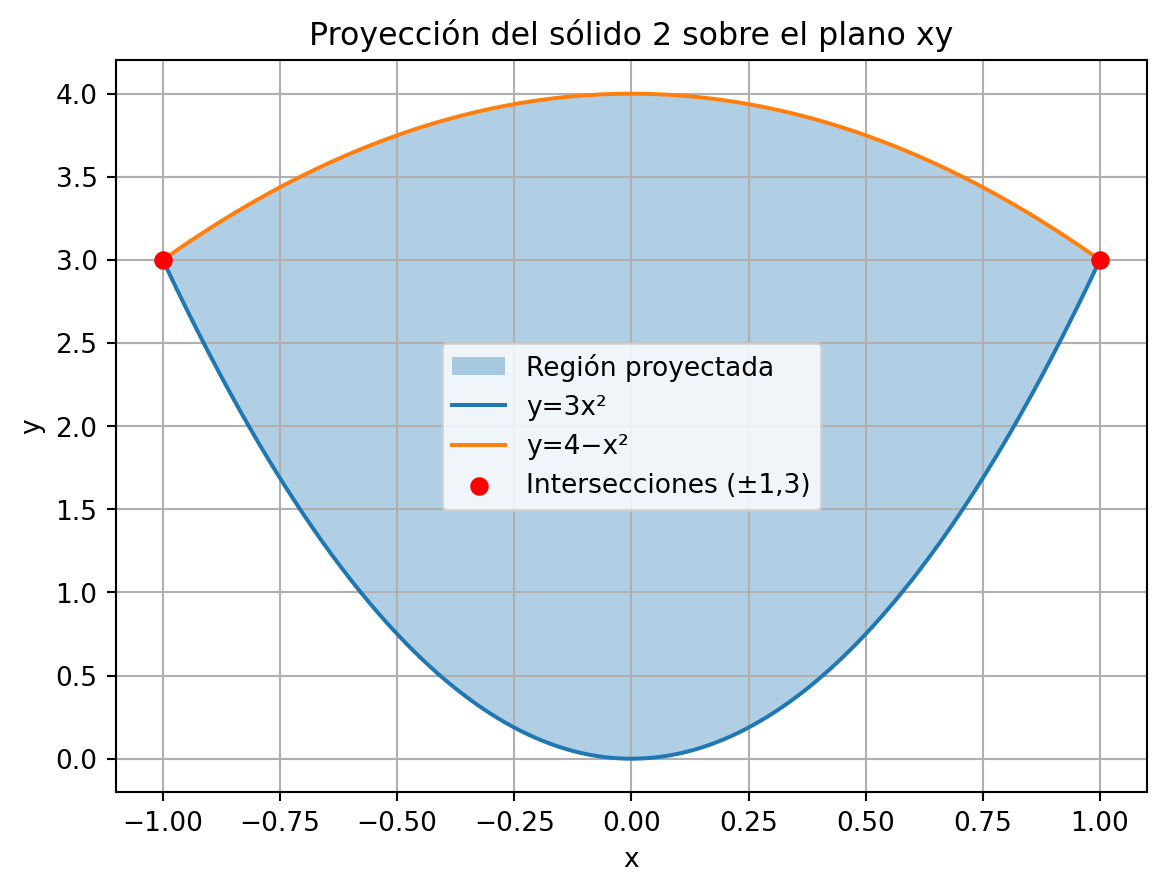
\includegraphics[width=0.82\textwidth]{graficas_taller_momento3/21_aplicacion_solid2_xy.png}
\caption{Proyección de la región del segundo sólido sobre el plano $xy$.}
\label{fig:aplicacion-proyeccion-2}
\end{figure}

\end{solution}


\chapter*{Conclusiones}
\addcontentsline{toc}{chapter}{Conclusiones}
La realización de este taller permitió consolidar el dominio conceptual y operativo de las herramientas del cálculo multivariado aplicadas a problemas tanto abstractos como de modelamiento espacial. Se evidenció con claridad la necesidad de adoptar criterios de mayor rigor analítico al trabajar en dimensiones superiores; en particular, se comprendió que el análisis de integrales en $\mathbb{R}^2$ y $\mathbb{R}^3$ exige descartar la dependencia de trayectorias arbitrarias o implementar acotamientos formales mediante el Teorema del Sándwich para certificar su convergencia, superando las limitaciones de los métodos del cálculo en una sola variable. Asimismo, el uso sistemático de trazas y curvas de nivel demostró ser un método fundamental para la reconstrucción geométrica precisa de superficies en el espacio tridimensional.\\


% Formato bibliografíco formal
\newpage
\addcontentsline{toc}{chapter}{Bibliografía}
\begin{thebibliography}{99}
\bibitem{ejemplo} James Stewart. \textit{Calculo de varias variables. Trascendentes tempranas}. 7ma Edicion .
\bibitem{ejemplo} Leithold Louis. \textit{El Calculo}. 7ma Edicion.
\bibitem{ejemplo} Ron Larson and Bruce Edwarsds. \textit{ Calculo}. 9na Edicion.
\end{thebibliography}

\end{document}